\documentclass[a4paper,10pt,oneside,openany]{memoir}

% Aesthetics
\chapterstyle{hangnum}
\renewcommand\contentsname{Table of Contents}

% Set language
\usepackage[british]{babel}

% bibliography
\usepackage[numbers]{natbib}

% Packages
\usepackage{xcolor}
\usepackage[T1]{fontenc}
\usepackage[utf8]{inputenc} % unicode support
\usepackage{tocbibind}
\usepackage{graphicx}
\graphicspath{ {figures/} }
\usepackage{pdfpages} % to import the front page
\usepackage{import}
\usepackage[justification=centering]{caption}% or e.g. [format=hang]
\usepackage{verbatim}
\usepackage{amsmath}

\usepackage{geometry} %% Alter margins on pages

\usepackage{adjustbox}

\usepackage{caption}
\usepackage{subcaption}
\usepackage{tabularx}
\usepackage{color}

% Set margin 
\setlrmarginsandblock{4.5cm}{4.5cm}{*}
\setulmarginsandblock{4.5cm}{*}{1}
\checkandfixthelayout 

% To list code blocks in latex
\usepackage{lstautogobble}
\usepackage{listings}
\lstset{
	language=C,                % choose the language of the code
%	numbers=left,                   % where to put the line-numbers
	stepnumber=1,                   % the step between two line-numbers.        
%	numbersep=5pt,                  % how far the line-numbers are from the code
	backgroundcolor=\color{white},  % choose the background color. You must add \usepackage{color}
	showspaces=false,               % show spaces adding particular underscores
	showstringspaces=false,         % underline spaces within strings
	showtabs=false,                 % show tabs within strings adding particular underscores
	tabsize=2,                      % sets default tabsize to 2 spaces
	captionpos=b,                   % sets the caption-position to bottom
	breaklines=true,                % sets automatic line breaking
	breakatwhitespace=true,         % sets if automatic breaks should only happen at whitespace
%	title=\lstname,                 % show the filename of files included with \lstinputlisting;
	autogobble=true
}

\lstdefinestyle{ttt}{
    basicstyle=\ttfamily,
  %columns=fullflexible,
    mathescape=true,
    literate={->}{$\rightarrow $}{1}
  }

\lstdefinestyle{csv}{
	xleftmargin=-2.5cm,
	xrightmargin=-2.5cm,
	belowskip=0pt,
	basicstyle=\scriptsize,
	stringstyle=\scriptsize,
	fontadjust=true}
% xml listings
\lstdefinestyle{XML}{ 
	columns=fullflexible, 
	basicstyle=\rmfamily, 
	commentstyle=\ttfamily\itshape\color{green!50!black}, 
	morestring=[s]{"}{"}, 
	morecomment=[s]{?}{?}, 
	morecomment=[s]{!--}{--}, 
	morecomment=[s]{!DOCTYPE}{]}, 
	moredelim=[s][\color{black}]{>}{<}, 
	moredelim=[s][\bfseries\color{black}]{\ }{=}, 
	stringstyle=\color{blue}, 
	identifierstyle=\bfseries\color{violet} 
}


%%%%%%%%%%%%%%%
% json listings starts
%%%%%%%%%%%%%%%%
\newcommand\JSONnumbervaluestyle{\color{blue}}
\newcommand\JSONstringvaluestyle{\color{red}}

% switch used as state variable
\newif\ifcolonfoundonthisline

\makeatletter

\lstdefinestyle{json}
{
	showstringspaces    = false,
	keywords            = {false,true},
	alsoletter          = 0123456789.,
	morestring          = [s]{"}{"},
	stringstyle         = \ifcolonfoundonthisline\JSONstringvaluestyle\fi,
	MoreSelectCharTable =%
	\lst@DefSaveDef{`:}\colon@json{\processColon@json},
	basicstyle          = \ttfamily,
	keywordstyle        = \ttfamily\bfseries,
}

% flip the switch if a colon is found in Pmode
\newcommand\processColon@json{%
	\colon@json%
	\ifnum\lst@mode=\lst@Pmode%
	\global\colonfoundonthislinetrue%
	\fi
}

\lst@AddToHook{Output}{%
	\ifcolonfoundonthisline%
	\ifnum\lst@mode=\lst@Pmode%
	\def\lst@thestyle{\JSONnumbervaluestyle}%
	\fi
	\fi
	%override by keyword style if a keyword is detected!
	\lsthk@DetectKeywords% 
}

% reset the switch at the end of line
\lst@AddToHook{EOL}%
{\global\colonfoundonthislinefalse}

\makeatother

%%%%%%%%%%%%%%%
% json listings ends
%%%%%%%%%%%%%%%%

\usepackage{float}
\usepackage[hidelinks]{hyperref}


% glossaries
\usepackage{glossaries}
\newacronym{mad}{MAD}{Median Absolute Deviation} % list of glossaries in a separate file

\newcounter{quote}

\newcommand\citea[1]{%
	(\citeauthor{#1},~\citeyear{#1})}

\newcommand\citeap[2]{%
	    \ifx&#1&%
	    % #1 is empty
	    (\citeauthor{#2},~\citeyear{#2})
	    \else
	    % #1 is nonempty
	    (\citeauthor{#2},~\citeyear{#2}:#1)%%
	    \fi
}
	
% enquote some text
\newcommand{\q}[1]{``#1''}
\newcommand{\qe}[1]{``\emph{#1}''}

% Commands
% Horizontal lines used for the Front Page Title
\newcommand{\HRule}{\rule{\linewidth}{0.5mm}}

\begin{document}

%\frontmatter{}

% Standard Frontpage
%TODO INCLUDE STANDARD FRONTPAGE
%\includepdf[pages={1}]{standardfrontpage2.pdf}

%TODO INCLUDE NORMAL FRONTPAGE
\begin{center}
  \thispagestyle{empty}

  % Header text
  \textsc{\LARGE IT University of Copenhagen}\\[0.5cm]
  \textsc{\Large  (Thesis)}\\[2cm]

  % Title in box
  \HRule\\[0.4cm]
  {\huge \bfseries Untitled Thesis Project \\ [0.4cm]}
  \HRule\\[3cm]

  % Author and supervisor
  \begin{tabular}{lr}
  	\textit{Authors:} \\
    Ans Uddin                     & \texttt{anud@itu.dk} \\
    \\
    \\
    \\
    \textit{Supervisor:}\\
    Willard Rafnsson \\
    \\
    \textit{Co-supervisor:}\\
    Carsten Schürmann\\
  \end{tabular}

  \vfill
  {\large February, 2018}
\end{center}



\pagenumbering{roman}
\setcounter{secnumdepth}{-1}
\frontmatter{}

\chapter{Abstract}

The thesis is a case study of secure implementation using the Information-Flow Control tool Paragon on top of the Matrix protocol. The implementation is a prototype inspired by Danish patient journals systems which requires end-to-end security. End-to-end security is the guarantee of confidentiality and integrity throughout the system. Matrix is a secure communication protocol that ensures confidentiality and integrity of information through end-to-end encryption. However encryption provides no such guarantees once the information is decrypted at the endpoints. Information-Flow Control is such a mechanism that can ensure confidentiality and integrity at the endpoints by enforcing security policies. Paragon is a Java based programming language with the ability to define and enforce security policies.

The thesis contributes with a interface between Paragon and Matrix allowing implementations with end-to-end security on top of Matrix.





\chapter{Acknowledgements}
\input{tex/Acknowledgements}

\pagebreak


\setcounter{tocdepth}{3}
\setcounter{secnumdepth}{3}

\tableofcontents*
\listoffigures
\listoftables







\mainmatter{}

\pagenumbering{arabic}
\chapter{Introduction}\label{intro}
\section{Data privacy and protection}

With GDPR becoming effective in 2018 the focus on data privacy is at its peak. 
Privacy violation is when sensitive data is exposed to unauthorized actors\cite{cwe}. OWASP top ten ranks \emph{sensitive data exposure} as 3rd biggest security threat\cite{owasp}. 

Recent cases of data leakage has put more attention on data privacy and protection. Some cases are due to poor security measures and could arguably have been prevented. Examples of cases are:

\begin{itemize}
	\item The infamous Facebook - Cambridge Analytica scandal. Third parties were able to collect data through Facebook Login API.
	\item Google Plus leak. 500.000 users private data was exposed to third parties through APIs\cite{googleplus}.
	\item Medicaid leak. A medical assistant had accessed patients' health records and exchanged mails with another employee containing the patients' private data\cite{medicaid}.  
\end{itemize}


%https://www.nytimes.com/2018/10/08/technology/google-plus-security-disclosure.html
%https://www.seattletimes.com/seattle-news/health/91000-state-medicaid-clients-warned-of-data-breach/

The cases above failed to achieve end-to-end security and the improper handling of sensitive data could have been prevented with appropriate security policies and enforcement technique that enforces these policies.

There is more awareness on how applications deal with data. This add extra concern to the programmer and the application about how sensitive data is handled and protected.  

The well-known security enforcement techniques like access controls, firewalls and encryption are inadequate alone and does not ensure end-to-end security\cite{Sabelfeld2003}.




%https://cwe.mitre.org/data/definitions/359.html


%OWASP top ten A3 sensitive data exposure


\section{Information Flow Control} % ikke teknisk. hvilke problemer løser ifc -> lave eksempeler med kode

There exist useful security enforcement mechanisms for protecting confidential information such as firewalls, encryption and access control. However, these mechanisms each have their drawbacks.

\begin{itemize}
	\item \emph{Access} control prevents unauthorized access to information but once access is granted there is no guarantee how that confidential information is handled.
	\item \emph{Firewall} limits communication from the outside hence isolate and protect information. Yet the firewall have no way of telling if the communication going through violates confidentiality.
	\item \emph{Encryption} secures information on a channel with only the endpoints being able to access that information. However there is no assurance that once the data is decrypted that the confidentiality of that information is ensured.
\end{itemize}

The mechanisms mentioned above all have in common that they lack control of how the information flows. Information-flow security aims at protecting confidentiality and integrity of information by enforcing security policies. Information-Flow Control allows the programmer to define and enforce policies in a language-based way\cite{Sabelfeld2003}. 



\section{Matrix}\label{matrix:intro}
Matrix is an open standard protocol for messaging over HTTP and synchronizing data. Matrix provides secure real-time communication over a decentralized federated network. Matrix secures data by providing end-to-end encryption.

Matrix cover use cases such as instant messaging, VoIP, Internet of Things communication and is generally applicable anywhere for subscribing and publishing data over standard HTTP API.
 
The fragmentation of IP communication is the problem Matrix essentially wants to solve. Making calls and messages between users needless of which app they use. However they define their longer term goal as \emph{"to act as a generic HTTP messaging and data synchronisation protocol for the whole web"}\cite{matrixfaq}.



%https://matrix.org/docs/guides/faq
%However in the presence of end-to-end encryption, apps can still leak through their application logic; a content-filtering chat bot running at the receiving end of an end-to-end encrypted connection can leak anything it receives from this connection. 



\section{The case study} % Challenges 

The goal of the case study is to make secure implementation of a prototype using Information-Flow Control. The case study will use Matrix as the communication channel and strengthen the security at the endpoints using IFC.

\subsection{Journal system}
The prototype implements a journal system and is loosely based on the Danish E-journal system.

%https://journalofethics.ama-assn.org/article/electronic-health-records-privacy-confidentiality-and-security/2012-09
Medical privacy is a well-known issue\cite{Rahim2013}. Sensitive data about patients needs to be handled carefully. In Denmark patients have access to their medical records through E-journal\cite{ejournal}. A patient's journal on E-journal is available for up to 90.000 different medical employees\cite{JP90000}. 

There are clear policies about who and under what conditions should access a journal. It is legally required that an employee accessing the journal must have the patient in care and that the lookup must be relevant for the employee. Safety measures have been applied through logging and audit trails with random sampling checks however they do not prevent access to journals. Any medical employee can access the patient journal and even if prevention mechanism were established there would be no limitation to what a medical employee could see once access was granted \cite{adgang}\cite{kontrol}. 

%Example of a being referred to a physician. A physician can access the patient journal but can see full history of the patient sessions. If the patient had psychiatric treatment it would be of no relevance to that medical employee. 

%https://www.sundhed.dk/borger/service/om-sundheddk/om-portalen/datasikkerhed/andres-dataadgang/adgang-til-sundhedsdata/

The mechanisms in the current journal system might restrain malicious intend. However it does not guarantee prevention of unintentional access or disclosure of information\cite{Harman2012}. 
What is missing is the enforcement of secure information flow policies. Unintentional access or disclosure of information can be prevented by enforcing policies that define secure information flow.

The prototype will model a simplified scenario of hospitals with different actors accessing a patient journal. The bulk of information on the journal system is extracted from newspaper articles hence there is a high uncertainty of how the system really works. Therefore many assumptions are made about the current system when programming the prototype.


%https://journalofethics.ama-assn.org/article/electronic-health-records-privacy-confidentiality-and-security/2012-09


%https://cwe.mitre.org/data/definitions/359.html

%https://www.version2.dk/artikel/e-journals-systemadministrator-vi-vaerner-patienternes-privatliv-1059692
%Vi kan ikke garantere, at alle bliver opdaget, men borgerne kan se i 'Min log', hvem der har været inde og se på deres data. Derudover laves der en auditering, hvor ca. fire procent af alle opslag undersøges, og der verificeres, om der har været en behandlerrelation.
%Loggen på sundhed.dk viser kun de tilgange til journalen der har været via netop sundhed.dk. Læger, apoteker m.m. har nemlig også en adgang til sundhed.dk hvor de kan slå folk op - og det bliver logget. Men loggen i sundhed.dk viser IKKE de opslag der sker i alle de andre systemer i sundhedsvæsenet, f.eks. patientjournal-systemerne. 
%https://www.version2.dk/artikel/90000-ansatte-har-adgang-til-patientjournaler-stikproever-er-eneste-kontrol-58628
%https://jyllands-posten.dk/indland/ECE6715461/op-imod-90000-ansatte-kan-kigge-i-din-journal/
%https://www.dr.dk/nyheder/regionale/sjaelland/it-systemer-snakker-ikke-godt-nok-sammen-risikerer-gaa-ud-over

\subsection{Scope} 
%Selvom jeg ikke kiggr på fx trafic analysis så er det vigtigt at nævne og påpege det ikkeer noget jeg løser.

% Clarify at the exam what is meant by the Matrix security model described in the project proposal 

% The goal of the thesis is not to reimplement Matrix using IFC tools. It is to use Matrix and analyze the security model and see what security guarentees and how we can improve security for the system that uses Matrix. 
The objective of the project is to do a secure implementation of the prototype described above. Secure exchange of patient journal is ensured using Matrix and the endpoints are secured using IFC.

A successful project is one that fulfills these criteria: 

\begin{itemize}
	\item Evaluation of Matrix security model
	\item Survey of IFC tools and selection of tool.
	\item Implement a prototype distributed system running on Matrix, using the chosen tools
	\item Demonstrate increased security guarantee with Matrix and IFC
\end{itemize}   


\subsection{Why Matrix?}
In the Digital Strategy 2016-2020 the Danish Agency of Digitisation defines initiative 7.2 as \emph{"Common standards for secure exchange of information"}. The large number of software systems in the Danish public sector has created a need for an uniform way of exchanging data across different application in a secure manner\cite{TheGovernment2016}. 

The initiative has similarities to the issue Matrix is trying to solve with fragmented IP communication. With Matrix security guarantees and their long term goal as a generic HTTP messaging protocol there is a strong case for using Matrix as a communication channel in this case study.


%Matrix gives security guarantees in term of end-to-end encryption and makes data exchange secure; however the end-points are still vulnerable. By using Matrix as the communication channel it gives gives a stronger security guarantee and adds complexity to the solution being developed using IFC tools. 
 
\section{Method}
 
 \section{Threat model}
 %adversary model
 The threat model is defined in the context of confidentiality and integrity.
 \begin{itemize}
 	\item The adversary has the ability to observe information sent over the network.
 	\item The adversary can generate input to the system .
 	\item The adversary can observe public output.   
 \end{itemize}
 
 % Dolev-yao model
 
 
 
\section{Contribution} %end-to-end security

The contributions to the field are the findings of secure implementation using Paragon and how they compare to similar findings from secure implementation with JIF.

The thesis also contributes with the interface created between Paragon and Matrix making it possible to develop other secure applications on top of secure communication channel Matrix provides. 

 
 
\section{Structure of thesis} % her kan nævnes den antagelse gøres 

Chapter \ref{background} sets the foundation for the thesis and introduces relevant information and background. Chapters \ref{analysis} analyzes the Matrix security model and survey IFC tools. Chapter \ref{design} goes in depth with design of the solution. The results are then presented and discussed in Chapter \ref{results}. The thesis is wrapped up in the conclusion section Chapter 6. 
 
\section{Summary}
There is more awareness on how applications deal with data. This add extra concern to the programmer and the application about how sensitive data is handled and protected. Encryption is an obvious way of ensuring confidentiality; Matrix is a tool that provides end-to-end encryption. However there is no guarantee of encryption of the data is decrypted. Information flow control is such mechanism that enforces security policies throughout the system.



\chapter{Evaluation of Matrix Security model}\label{evaluationchapter}

This chapter consists of two parts. The first part will provide an evaluation of the Matrix security and relies on the paper \emph{SoK: Secure Messaging} \cite{sok} and \emph{The Olm Cryptographic Review} by NCC Group \cite{ncc}. 

The second part provides a preliminary analysis of some IFC tools, the selection of Paragon and the rationale behind it.



Section \ref{evaluationofmatrix} provides an evaluation of the Matrix security model. The security model is evaluated in the context of a secure messaging system.  
The paper \emph{SoK: Secure Messaging} describes a evaluation framework for evaluating secure messaging systems. They define several security properties related to such systems \cite{sok} which will be presented.


All secure messaging systems with end-to-end encryption are based on the Double Ratchet algorithm from the Signal Protocol which will also be described.


Finally the architecture of Matrix and concepts related to Information-Flow Control will be introduced.

\section{Information security}

Information security is the discipline of protecting information. The key principles in information security are expressed through the CIA model. For a system to be secure these principles should be guaranteed \cite{michael2012}.

\begin{figure}[H]
	\centering
	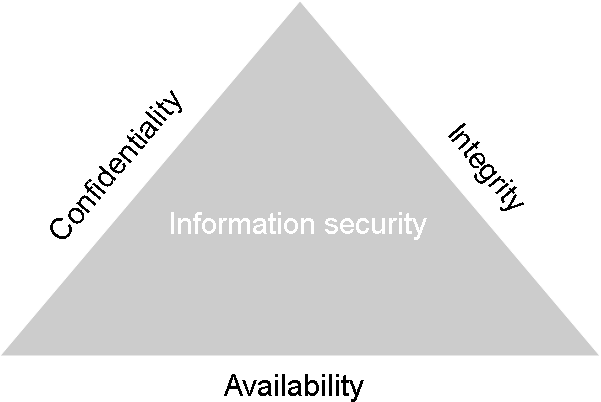
\includegraphics[width=10cm]{figures/cia.png}
	\caption{CIA triad}
	\label{fig:CIA triad}
\end{figure}


\subparagraph{Confidentiality}
Confidentiality is keeping information secret from unauthorized people. This is a major goal in information security. Encryption and access control are common ways of ensuring confidentiality \cite{michael2012}.

In a secure messaging system confidentiality would be guaranteed if the message being sent is only readable by the recipient and no one else \cite{sok}.

\subparagraph{Integrity}
Integrity is providing that information is unaltered and can only be changed by authorized people. If information is intercepted and changed during transit it would be a violation of integrity \cite{michael2012}.  
More specifically for a secure messaging it would mean that no altered message is accepted by the recipient \cite{sok}.

\subparagraph{Availability}
Making sure that information is accessible to authorized people is the goal of availability. Denial of Service attack \footnote{https://en.wikipedia.org/wiki/Denial-of-service\_attack} are common attacks targeting availability. 

Availability is generally more related to the system being available where the information itself plays a minor role \cite{michael2012}.
\\
\\
Depending on the type of system other properties must be satisfied as well. 


\subsection{Security properties}
The goal in a secure messaging system is to protect the messages being sent. The following properties are used to evaluate Matrix in section \ref{evaluationofmatrix}. 


\subparagraph{Authentication}
When a message is received the participant can verify that the message was sent from the actual sender. Furthermore a participant will receive evidence from a participant in a conversation that hey hold a known long-term secret. 



\subparagraph{Perfect Forward Secrecy}
If all keys are compromised than the decryption of any previously sent message should not be possible. Hence all previous messages would be secure however all future messages would be insecure 

\begin{figure}[H]
	\centering
	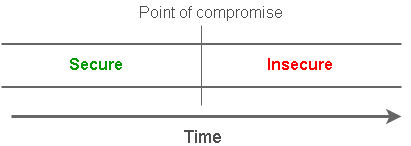
\includegraphics[width=10cm]{figures/forwardsecrecy.png}
	\caption{Forward secrecy}
	\label{fig:forward}
\end{figure}

\subparagraph{Backward secrecy}
If all keys are compromised than the decryption of \emph{future} messages should be possible. This property also goes by the names \emph{future secrecy} and \emph{post compromise security}. 

\begin{figure}[H]
	\centering
	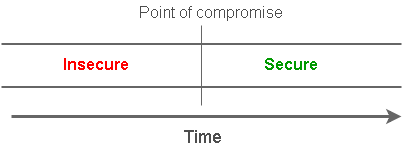
\includegraphics[width=10cm]{figures/backwardsecrecy.png}
	\caption{Backward secrecy}
	\label{fig:backward}
\end{figure}


\subsubsection{Other security properties}


\subparagraph{Participant Consistency} 
Whenever a message is accepted by a participant all participants are guaranteed to have identical view of the participant list.

\subparagraph{Destination Validation}
When a participant receives a message it can be verified that the participant was the intended recipient.

\subparagraph{Anonymity Preserving} 
The anonymity of the participants should be preserved and not linking any key identifiers.

\subparagraph{Speaker Consistency} 
There is consensus among the participants on the sequence of messages they receive by each participant. There might be a mechanism for checking consistency whenever a message is sent or after it has been received.

\subparagraph{Causality Preserving}
Messages must not be displayed before the message that originally precedes it has been displayed.

\subparagraph{Global Transcript} 
A global order where all messages are viewed in the same order for all participants.

\subparagraph{Deniability}
Deniability is a property where other participants cannot confirm that the message being sent was from the sender. Yet during the conversation there will be assurance for the recipient that the message being sent was authentic and sent by the sender \cite{sok}.

\begin{itemize}
	\item \emph{Message Unlinkability:} A deniability property that gives no guarantees that if a participant sent a message that other messages was sent by that participant as well. 
	\item \emph{Message Repudiation:} It can not be proved that a message was authored by a participant given the conversation transcript and all cryptographic key material. 
	\item \emph{Participant Repudiation:} It can not be proved that a participant was in a group conversation without his conversation transcript and cryptographic key material. 
\end{itemize}

The following properties are also defined in the paper \emph{SoK: Secure Messaging} but are less relevant for security.

\subparagraph{Group}

\begin{itemize}
	\item \emph{Computational Equality:} The computational load is equal for all participants.
	\item \emph{Trust Equality:} There is equal trust among all participants. 
	\item \emph{Subgroup messaging:} In the same conversation a participant can send messages to a subset of the participants.
	\item \emph{Contractible Membership:} When a participant leaves a conversation the protocol does not need to restart.
	\item \emph{Expandable Membership:} When a participant joins a conversation the protocol does not need to restart.
\end{itemize}

\subparagraph{Adoption}

\begin{itemize}
	\item \emph{Out-of-Order Resilient:} Messages received out-of-order should be accessible when received.
	\item \emph{Dropped Message Resilient:} On a unreliable network messages might be dropped in transit however it should not prevent decryption of future messages.
	\item \emph{Asynchronous:} Messages can be sent securely to recipients while they are offline.
	\item \emph{Multi-Device Support:} A participant can have multiple devices in a conversation and each device must be synchronized and should have the same historical conversation view
	\item \emph{No Additional Service:} There is no requirement of additional infrastructure being setup other than the participants. 
\end{itemize}




\section{Matrix}

Matrix is an open standard protocol for messaging over HTTP and synchronizing data. Matrix provides secure real-time communication over a decentralized federated network with eventual consistency. Matrix cover use cases such as instant messaging, VoIP, Internet of Things communication and is generally applicable anywhere for subscribing and publishing data over standard HTTP API.

%Any kind of json can be published to a room \cite{matrixvideoiot}.
% 3:10


% https://www.youtube.com/watch?v=-ofZMnKkp_Y 5:00 , 18:30

\subsection{How does it work?}

Matrix defines a conceptual place \emph{room} where data can be published and subscribed to. A room is shared and replicated among multiple \emph{homeservers}. The example shown in figure \ref{fig:matrix1} is a conversation in a room between three clients on different homeservers. 

In the example Alice starts by sending a message to the room. When Alice sends a message it is send to her homeserver. Each homeserver stores messages in a \emph{directed acyclic graph} called an \emph{event graph}. The message send by Alice is added to the event graph and is linked to most recent message(s) in the graph. The message is then signed with the signtatures of all previous messages by Alice's homeserver in order to make it tamper-proof. Finally the homeserver relays the message to the Bob's and Charlie's homeservers.

Upon receiving the message the other homeservers validates the message and then adds it to their own event graph. The message now persists in Bob's and Charlie's servers and can be retrieved from Bob's and Charlie's clients.

\begin{figure}[H]
	\centering
	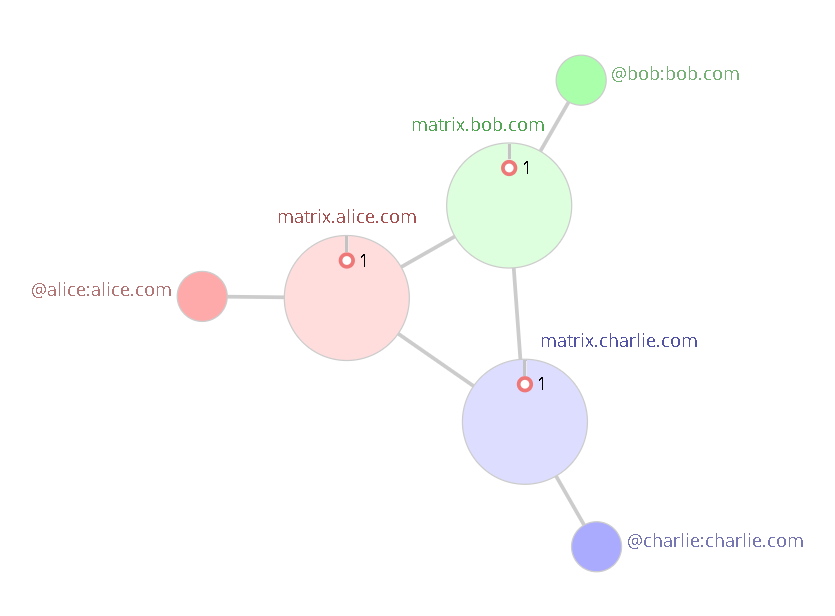
\includegraphics[width=9cm]{figures/matrix1.png}
	\caption{ Matrix \cite{matrixhome}.}
	\label{fig:matrix1}
\end{figure}

Bob replies to Alice's message and is first send to the homeserver and linked to Alice's message in the event graph. At the same time Charlie also send a reply and an inconsistency occurs as depicted in figure \ref{fig:matrix2}.


\begin{figure}[H]
	\centering
	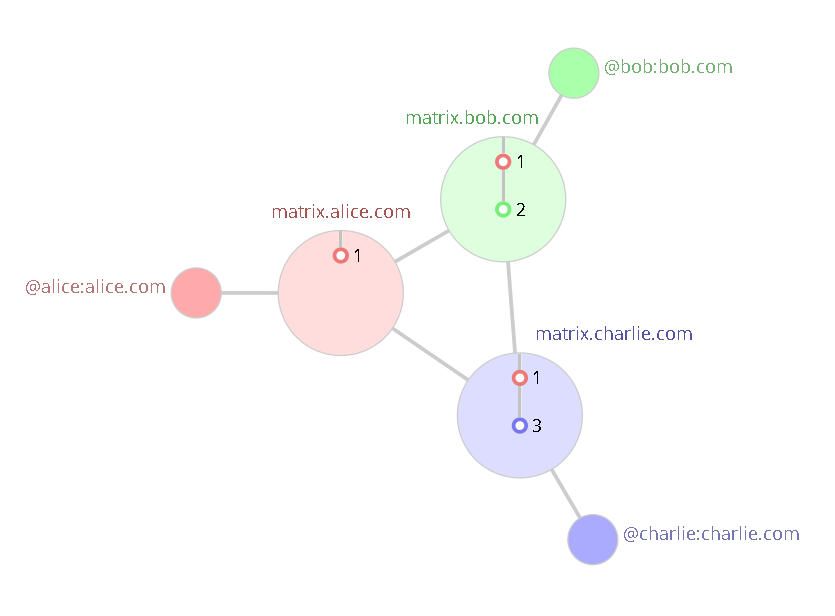
\includegraphics[width=9cm]{figures/matrix2.png}
	\caption{ Matrix \cite{matrixhome}.}
	\label{fig:matrix2}
\end{figure}


Bob's message arrives first to Alice and Charlie's homeservers. Alice adds the message to her own event graph and has a view that is consistent with Bob's. Charlie adds the message to the event graph; Bob's message precedes Alice's message hence message 2 and 3 are linked to message 1 shown in figure \ref{fig:matrix3};


\begin{figure}[H]
	\centering
	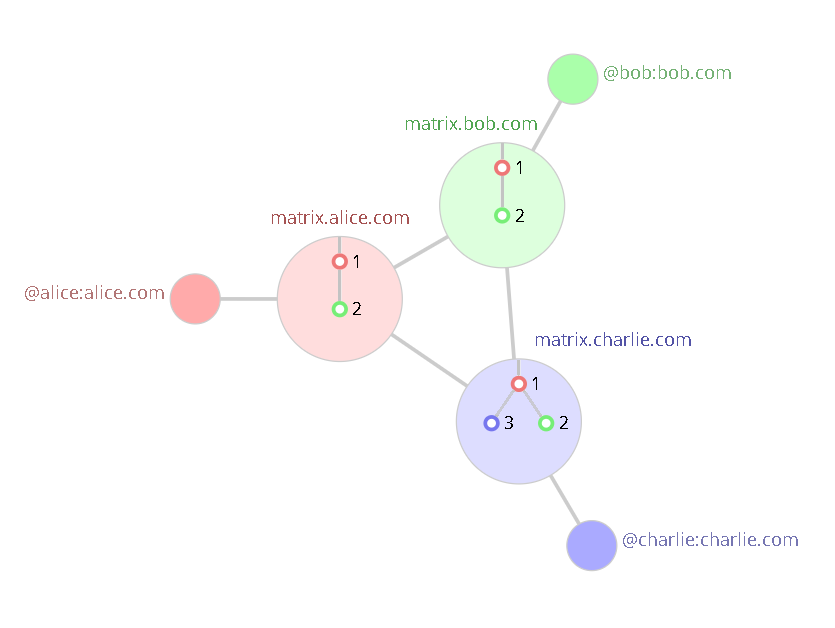
\includegraphics[width=9cm]{figures/matrix3.png}
	\caption{ Matrix \cite{matrixhome}.}
	\label{fig:matrix3}
\end{figure}


The other homeservers then receive Charlie's message and is added to their event graph. The room is yet again in sync and all the homeservers have a consistent view of the room.


\begin{figure}[H]
	\centering
	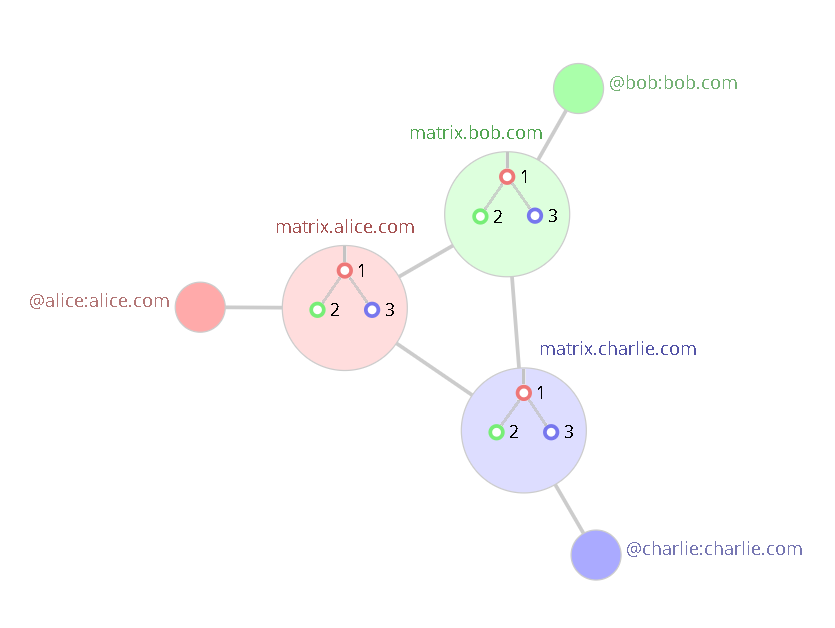
\includegraphics[width=9cm]{figures/matrix4.png}
	\caption{ Matrix \cite{matrixhome}.}
	\label{fig:matrix4}
\end{figure}

Alice sends a new message and is linked to the most recent unlinked objects (both Bob's and Charlie's). The message is then relayed to the other homeservers. The split in the event graph is merged. This example also shows how Matrix provides eventual consistency.

\begin{figure}[H]
	\centering
	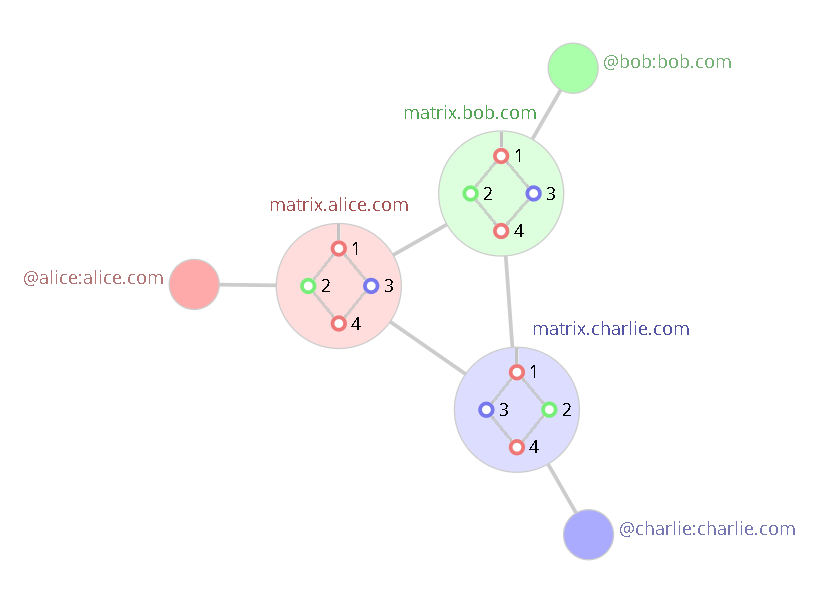
\includegraphics[width=9cm]{figures/matrix5.png}
	\caption{ Matrix \cite{matrixhome}.}
	\label{fig:matrix5}
\end{figure}

%In the example above the message is represnted by a JSON object and could be of any kind of object.


\subsection{Architecture} \label{matrix:architecture}
The previous section introduced the notion of a\emph{room} which clients sends messages to. The messages being in Matrix are actually JSON objects called \emph{events}. The events can be of any kind of structure hence it is not limited to messaging. Events are stored at homeservers and the communication history for a room is modelled using \emph{directed acyclic graph} called\emph{event graphs}. Matrix provides a specification for Client-Server API which is used for sending and synchronizing events between the client and its belonging homeserver. Matrix also provides specification for a Server-Server API which synchronizes data among homeservers with eventual consistency. The synchronization process between homeservers is defined by the term \emph{Federation} \cite{matrixspec}. 


\begin{figure}[H]
	\centering
	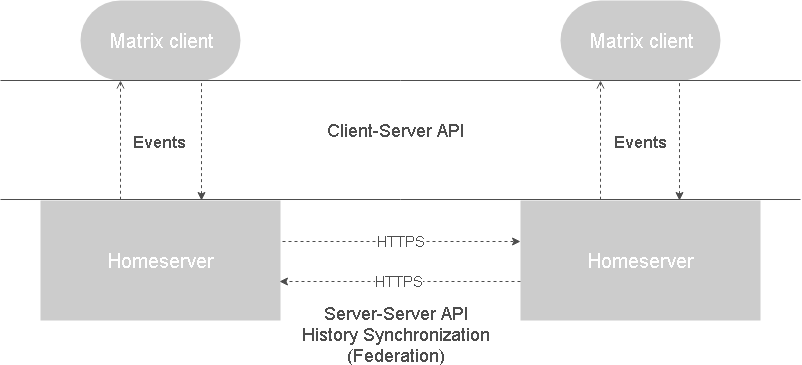
\includegraphics[width=11cm]{figures/matrix_architecture.png}
	\caption{ Matrix conceptual architecture \cite{matrixspec}.}
	\label{fig:matrix_architecture}
\end{figure}


As previously mentioned a room is a conceptual place for sending and receiving events with the room data being distributed over each homeserver. Each room is uniquely identified by a \emph{Room ID}. The figure \ref{fig:matrix_room} shows how events are send and received from a room.



\begin{figure}[H]
	\centering
	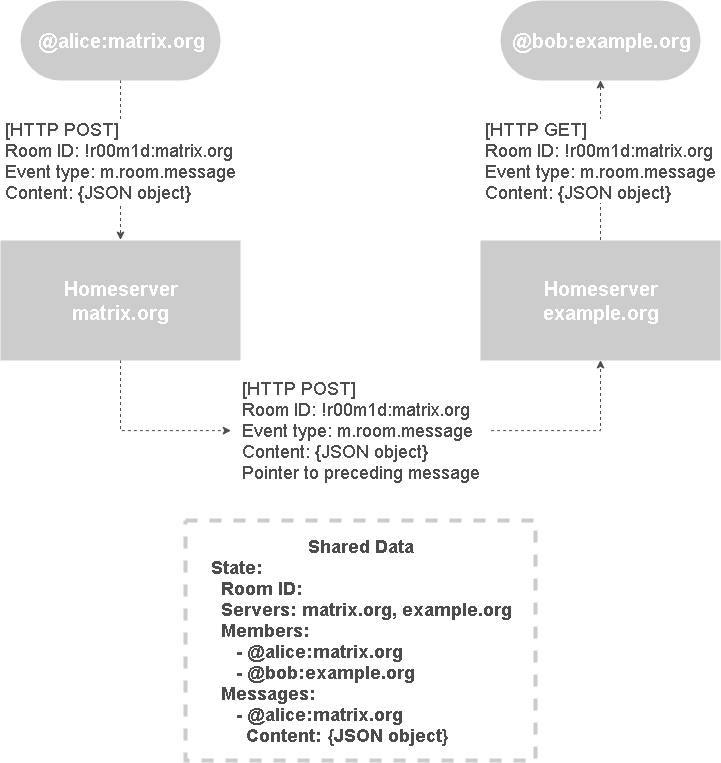
\includegraphics[width=10cm]{figures/matrix_room.png}
	\caption{ Matrix conceptual architecture \cite{matrixspec}.}
	\label{fig:matrix_room}
\end{figure}

\subsubsection{Event}

Every data exchange in Matrix is an event. Events are used to express state changes in a room as well as messages being sent. An event has a type used to differ between what kind of event is being sent and what kind of data it might hold. Matrix comes with reserved name spaces; \emph{m.room.message} is a type for instant messaging. The following is an example of a event of type \emph{m.room.message} \cite{matrixspec}.


\begin{lstlisting}[style=json]
{
	"content": {
		"body": "Hello world!",
		"msgtype": "m.text"
	},
	"room_id": "!wfgy43Sg4a:matrix.org",
	"sender": "@bob:matrix.org",
	"event_id": "$asfDuShaf7Gafaw:matrix.org",
	"type": "m.room.message"
}
\end{lstlisting}

The specification is open for defining custom types which can express any kind of data one might want to exchange \cite{typeofevent}.


\subsection{Matrix specification}
Matrix has two main API specifications; Client/Server API and Federated API. Any Matrix SDK implements the API defined at the Client/Server API specification. If a custom homeserver was to be developed from scratch it would have to conform to the Federated API to be able to be a part of Matrix. 

\subparagraph{Client/Server API}
For clients to send and receive messages the Client/Server API is used. The API mainly provides specification for:

\begin{itemize}
	\item Sending and receiving messages
	\item Configure rooms
	\item Synchronize historical conversation
\end{itemize}

There exist several SDKs implementing the API.  

\subsection{End-to-end Encryption}
Security is a high priority for Matrix design. Especially with the decentralized architecture with data being replicated over a federation federation of servers. Matrix provides security guarantees through end-to-end encryption using Olm and Megolm cryptographic ratchet. Olm is based on the Double Ratchet algorithm and Megolm is an extension for secure group communication. Olm and Megolm are examined in section \ref{matrixeval}.



\subsection{Concepts}



\subsubsection{Diffie-Hellman Key Exchange}

Diffie-Hellman is a key exchange protocol to establish a shared secret over an insecure channel. Public information is send over an insecure and using asymmetric keys two parties can derive the same shared key.


The first step is to agree on some public values. Either of the parties start the protocol by picking a large prime \emph{p} and a integer \emph{g} then the values are sent over the insecure channel.  

\begin{figure}[H]
	\hspace*{-1cm} 
	\centering
	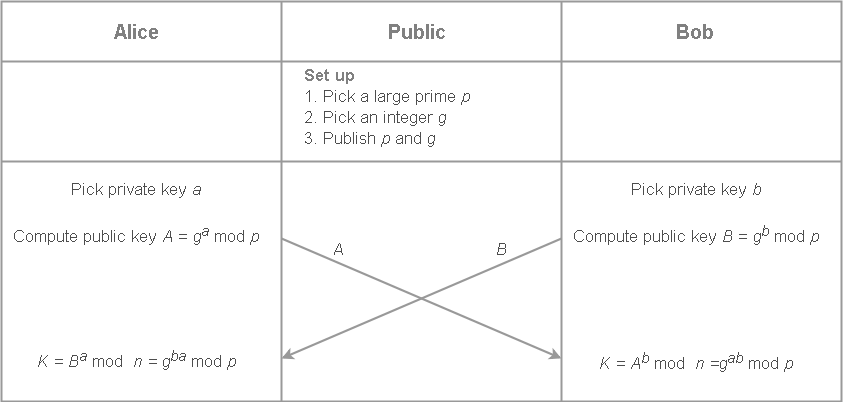
\includegraphics[width=14cm]{figures/dh.png}
	\caption{Simple Diffie-Hellman Key Exchange}
	\label{fig:dh}
\end{figure}

Alice and Bob will each pick a private key value and compute a public key value. The computed key value is sent over the insecure channel and Alice and Bob will both perform the same computation as previously \cite{crypto101}.


The Diffie-Hellman is vulnerable to man in the middle attack since there is no authentication taking place. There exist a solution to this problem using asymmetric key pairs and signing the messages being sent \cite{crypto101}.

\subsubsection{Key Derivation function}

Assume a secret key is established between two parties and is used to encrypt messages and exchange them over an insecure channel. An adversary listening might store all the messages being send even though he is not able to read them. However at some point he manages to compromise the secret key hence being able to decrypting every message ever sent.

To overcome the above scenario ephemeral keys are used. Such keys are short lived and are discarded after use.   

New secret keys can be generated using a \emph{Key Derivation Function} (KDF).
A KDF is a one way function that derives one or more randomized secret keys based on a secret key (or multuple) and optionally some input value \cite{crypto101}. Figure \ref{fig:kdf} illustrates this.

\begin{figure}[H] 
	\centering
	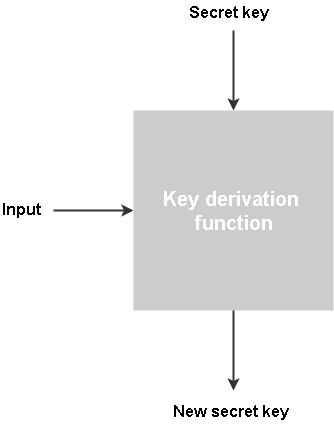
\includegraphics[width=8cm]{figures/kdf.png}
	\caption{Key derivation function}
	\label{fig:kdf}
\end{figure}


A core concept in the Double Ratchet algorithm is KDF chains which build a chain of secret keys using KDF \cite{doubleratchet}. 


\subsubsection{Signal Protocol}

The Signal Protocol provides end-to-end encryption and was developed in 2013 and was first introduced in the app TextSecure\footnote{https://en.wikipedia.org/wiki/TextSecure}.

The Signal Protocol consists of two parts; The \emph{Triple Diffie-Hellman protocol} (TripleDH) and the Double Ratchet algorithm.

\paragraph{Triple Diffie-Hellman protocol}\label{tripledh}
Before the Double Ratchet algorithm can be used the two parties communicating need to agree on a shared secret key. In the Signal protocol this is achieved with Triple Diffie-Hellman protocol \emph{(TripleDH)}.

The Triple Diffie-Hellman protocol is a \emph{key agreement protocol}. It involves a server and two parties; Alice and Bob. 

The TripleDH protocol is characterized by three phases:

\begin{enumerate}
	\item \emph{Publishing keys:} A identity key and several prekeys belonging to Bob is published by him to a server.
	\item \emph{Sending initial message:} Alice sends an initial message to Bob. A prekey bundle is obtained by Alice from the server in order to send an initial message to Bob.
	\item \emph{Receiving initial message:} Alice's message is received and processed by Bob.
\end{enumerate}


\paragraph{Double Ratchet algorithm}

After a shared secret key has been established the Double Ratchet algorithm can then be used to send and receive encrypted messages.

Each party has three chains; root chain, sender chain and receive chain. The chains are KDF chains and will take two keys as input (a KDF chain key and some other input key) and output new two keys (a new KDF chain key and some other output key). The KDF chain is illustrated in figure \ref{symkeyratchet}.

The algorithm has a \emph{Diffie-Hellman ratchet} step and \emph{symmetric ratchet} step and the chains are used across both steps.

\begin{itemize}
	\item \emph{Diffie-Hellman ratchet:} The parties exchanges new Diffie-Hellman public keys with the messages being sent. New secrets are then derived using Diffie-Hellman (DH). The secret that DH outputs is used as input to the root chain. The root chain then output new chain keys for the receiving and sending chains. 
	
	\item \emph{Symmetric ratchet:} The sending and receiving chains uses the chain keys derived from the root chain and for each message sent and received the chains are advanced. The output from the receiving and sending chains are keys for encrypting or decrypting messages. 
\end{itemize}


\subparagraph{Symmetric ratchet}
The symmetric ratchet provides message key through the receiving and sending chains. A message key is used for encryption or decryption of a message.

In the symmetric ratchet a single ratchet step is the calculation of the next key chain and message key. The inputs are the current chain key and a constant. Figure \ref{fig:symkeyratchet} illustrates two steps in a symmetric ratchet.

\emph{Forward secrecy} is provided since KDF is a one-way function and it is not possible to go backward and get the input chain key from the output chain key. However since the other input is simply a constant all future keys chain keys and message keys can be derived from an older chain key more specifically there is lack of backward secrecy.


\begin{figure}[H]
	\centering
	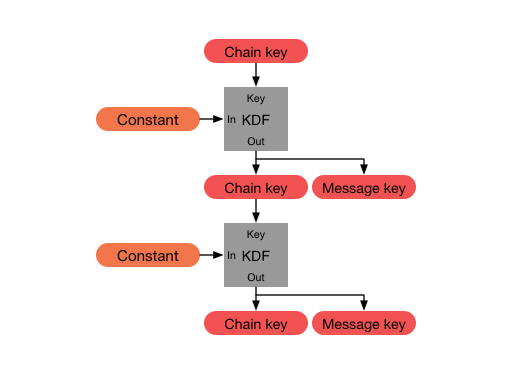
\includegraphics[width=10cm]{figures/symmetrickeyratchet.png}
	\caption{Symmetric key ratchet \cite{doubleratchet}.}
	\label{fig:symkeyratchet}
\end{figure}


\newpage
\subparagraph{Diffie-Hellman ratchet}

Double ratchet provides backward secrecy by comining the Symmetric ratchet with a Diffie-Hellman ratchet hence the name \emph{Double Ratchet}.

Every message from either party begins with a header which contains the sender's current ratchet public key. Whenever a new ratchet public key is received a new ratchet key pair is generated; a secret is derived through Diffie-Hellman with the input being the received ratchet public key and the ratchet private key from the new generated key pair.

Alice starts a conversation with Bob and uses his published public key as a ratchet public key. Alice then generates a new ratchet key pair and derives a shared secret key using Diffie-Hellman and would that as input to her \emph{sending chain}. Alice then sends her new ratchet public key to Bob. At the receiving end Bob derives the same shared secret which would be the input to his \emph{receiving chain}. Alice's sending chain and Bob's receiving chain share the same secret hence he can derive the message key and decrypt the message sent from Alice. When Bob sends a reply to Alice he would generate a new ratchet key pair and derive a new secret which would be input to his \emph{sending chain}.

Figure \ref{fig:dhratchet1} shows an ongoing message exchange with new secrets being derived and the sending and receiving chains being advanced.

\begin{figure}[H]
	\centering
	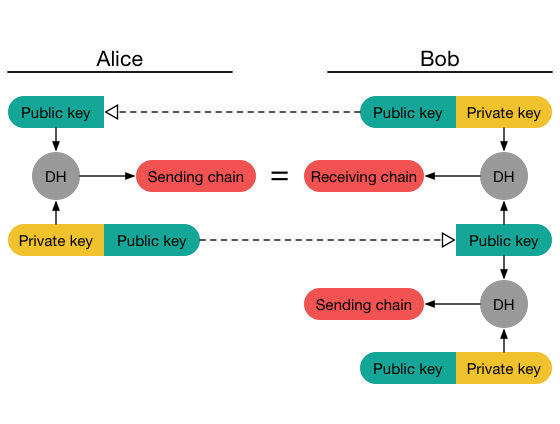
\includegraphics[width=9cm]{figures/dhratchet5.png}
	\caption{Diffie-Hellman ratchet \cite{doubleratchet}.}
	\label{fig:dhratchet1}
\end{figure}


When Alice receive the reply from Bob she would perform the exact same steps. This ultimately results in a continous loop of generating new ratchet key pairs and using Diffie-Hellman to derive the same shared secret key. A continuation is shown in figure \ref{fig:dhratchet2}

\begin{figure}[H]
	\centering
	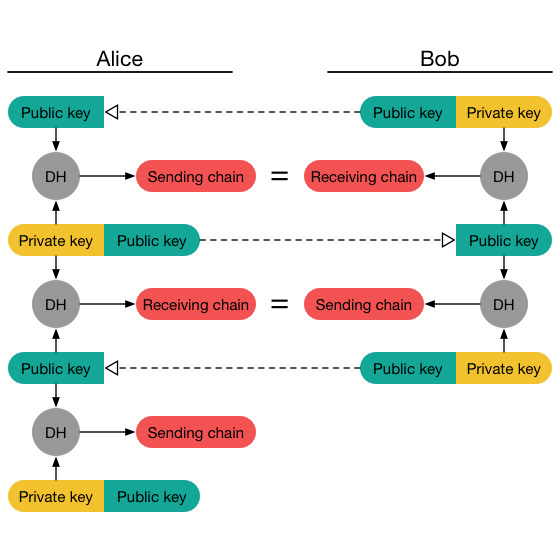
\includegraphics[width=9cm]{figures/dhratchet6.png}
	\caption{Continuation of Diffie-Hellman ratchet  \cite{doubleratchet}.}
	\label{fig:dhratchet2}
\end{figure}


As mentioned in the beginning of the Double Ratchet section the Diffie-Hellman ratchet does have a root chain which would provide inputs to the sending and receiving chains. A more correct view of the process in Diffie-Hellman is shown in figure \ref{fig:dhratchetcon}. 


\begin{figure}[H]
	\centering
	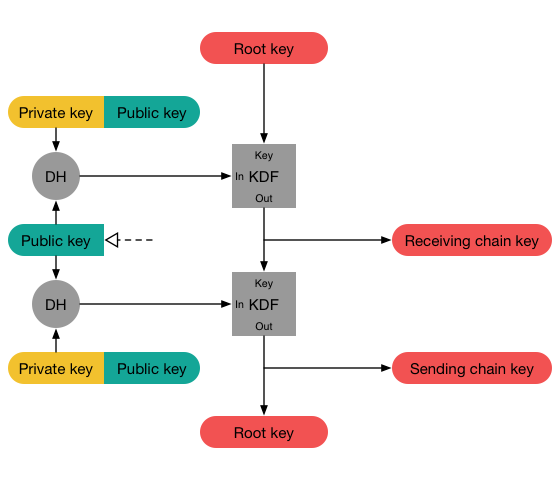
\includegraphics[width=9cm]{figures/dhratchet7.png}
	\caption{Diffie-Hellman ratchet 7 \cite{doubleratchet}.}
	\label{fig:dhratchetcon}
\end{figure}

\paragraph{Double ratchet}

When combining Diffie-Hellman ratchet and symmetric-key ratchet the result is the Double ratchet.

\begin{itemize}
	\item When sending or receiving a message the corresponding message key is derived by performing a symmetric-key ratchet step.
	\item Upon receiving a new ratchet public key the Diffie-Hellman ratchet step performed right before the symmetric-key ratchet step with the goal of replacing old chain keys with new ones.  
\end{itemize}

Assume that the message exchanged is a continuation from the TripleDH key exchange described in section \ref{tripledh}. Alice had sent an initial message. The initial ratchet public key would be Bob's signed prekey \emph{SPK\textsubscript{B}} and the new ratchet key pair would be the Alice's ephemeral key pair that she generated. Alice calculated a shared secret which is the \emph{root key}. She then generates a new ratchet key pair and takes the output from Diffie-Hellman and use it as input for the \emph{root chain}. The root chain then outputs a new root key \emph{RK} and a sending chain key {CK}.

The figure \ref{doubleratchet1} depicts this with a view of Alice's chains.


\begin{figure}[H]
	\centering
	
\includegraphics[width=10cm]{figures/doubleratchet1.png}
	\caption{Double ratchet 1 \cite{doubleratchet}.}
	\label{fig:doubleratchet1}
\end{figure}

When Alice then sends a message \emph{A1} the symmetric-key ratchet step will return a new chain key and a message key. The message can then be encrypted with the message key.

\begin{figure}[H]
	\centering
	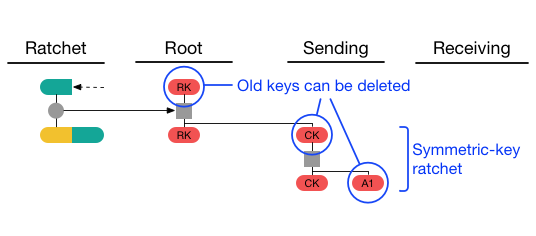
\includegraphics[width=10cm]{figures/doubleratchet2.png}
	\caption{Double ratchet 2 \cite{doubleratchet}.}
	\label{fig:doubleratchet2}
\end{figure}

Next Alice receives a message \emph{B1} from Bob. The message header contains a new ratchet public key and a Diffie-Hellman ratchet step is performed. New sending and receiving chain keys are derived and followed by a symmetric-key ratchet step to derive the receiving message key to decrypt the message.

\begin{figure}[H]
	\centering
	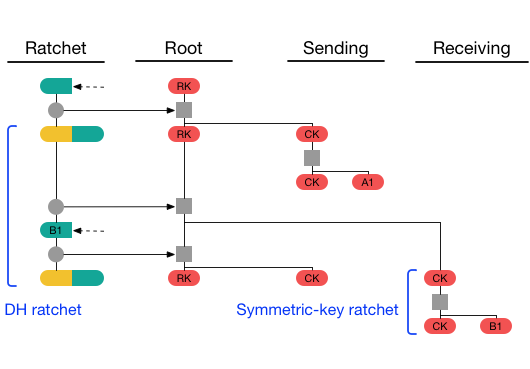
\includegraphics[width=10cm]{figures/doubleratchet3.png}
	\caption{Double ratchet 3 \cite{doubleratchet}.}
	\label{fig:doubleratchet3}
\end{figure}






% This chapter will present the criteria \emph{evaluation of Matrix security model}

\section{Evaluation of Matrix security model}\label{evaluationofmatrix}
The security of matrix will be evaluated in the context of secure messaging. An evaluation framework has been proposed in the paper \emph{SoK: Secure messaging} which the evaluation will be loosely based on. 

The evaluation framework covers several areas with \emph{conversation security} being the most relevant for this evaluation. The area \emph{conversation security} describes three categories; \emph{Security and Privacy}, \emph{Adoption}, and \emph{Group Chat}. Obviously the most relevant category for the evaluation is \emph{Security and Privacy}

\subsection{Threat model}
For secure messaging the evaluation framework defines a threat model with three types of adversaries. Note that an adversary can be of several types:

\begin{itemize}
	\item \emph{Local adversary:} The adversary is in control of the local network.
	\item \emph{Global adversary:} The adversary is in control of great portions of the Internet 
	\item \emph{Service providers:} A potential adversary for messaging systems with centralized infrastructure.
\end{itemize}

In the messaging system the adversary may be a participant with the following properties:

\begin{itemize}
	\item An adversary can start a conversation.
	\item An adversary can send messages.
	\item An adversary can perform any other action that a participant is capable of.
\end{itemize}

Furthermore it is assumed that the system's endpoints are secure \cite{sok}.

This evaluation will inherit the described threat model.

\subsection{The Signal Protocol}
Matrix provides end-to-end encryption by using the Olm and Megolm library with the former being an implementation of the Double Ratchet algorithm also known as the Signal Protocol, and the latter being the algorithm used for group chat. 

Olm is used for securely exchanging message keys/session keys during group chat and is vital part of the end-to-end encryption in Matrix.

Before the Matrix protocol is evaluated the Signal Protocol will be considered. The Signal Protocol is described in section xx. 

Section xx provides a list of security properties relevant for \emph{conversation security}. These security properties is used for evaluating a secure messaging protocol such as the Signal Protocol.
%Any messaging application that provides end-to-end encryption is likely an implementation of  the protocol 

The table below shows an evaluation of the Signal Protocol (previously known as TextSecure) \cite{sok}. 

\begin{figure}[H]
	\hspace*{-1.7cm} 
	\centering
	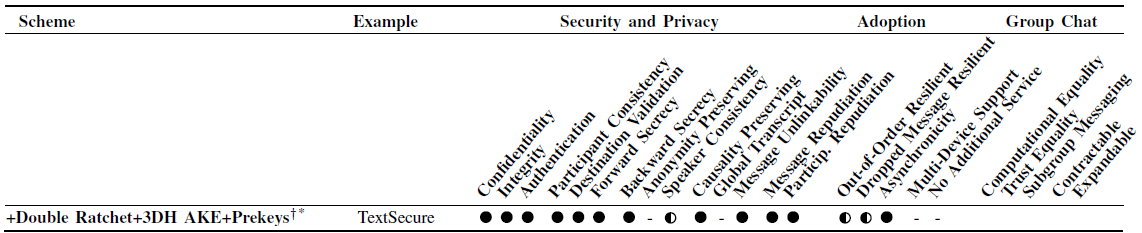
\includegraphics[width=16cm]{figures/framework_signal.png}
	\caption{Evaluation of Signal (TextSecure) \cite{sok}.}
	\label{fig:framework_signal}
\end{figure}


%Explain how they provide the properties or why they don't


\subparagraph{Confidentiality} When a message is sent using the Signal Protocol then only the intended recipient can read the message. The senders sending ratchet and receivers receiving ratchet will derive the same message key hence only the two parties will be able to encrypt the messages. 

\subparagraph{Integrity} The receiver will only accept a message if it is successfully decrypted hence if in transit a message was modified then the message would be rejected.

\subparagraph{Authentication} The decryption of a message also gives authentication guarantees since only the intended recipient could compute the message key.

\subparagraph{Forward secrecy} The symmetric ratchet ensures forward secrecy. If a chain session key is compromised then the previous keys can not be generated since the ratchet is one way cryptographic hash function hence secrecy is provided for all previous send messages.  

\subparagraph{Backward secrecy} Diffie-Hellman ratchet have the self-healing property and will generate a new chain session key for the symmetric ratchet hence if a chain key is compromised then secrecy for future messages is still provided because a new chain ratchet key will be generated.

\subparagraph{Anonymity preserving}

Anonymity preservation is lost in the Signal Protocol since the initial key agreement requires long-term public keys hence making them observable during Triple-DH. However \textbf{\emph{participant consistency}} is provided by Triple-DH \cite{sok}. %How?
%Without participant consistency, identity misbinding attacks might be possible. Unknown key share attack

\subparagraph{Speaker consistency}
This property is partially provided through the key evolution of the ratchets. If a message is dropped then it is not possible to generate message keys for future messages. This also makes the protocol have the property \textbf{\emph{Causality Preserving}} and partially have the property \emph{\textbf{Dropped message resilence}}. It will also not go unnoticed if a message is received out of order since this will result in the message's key being an unexpected key. Hence the recipient have to store expired keys to decrypt delayed messages. This makes the property \emph{\textbf{Out-of-order resilient}} only partially provided \cite{sok}.

\subparagraph{Global transcript} 
In an asynchrounous messaging protocol there is no global transcript. Both participants have to be online to receive messages hence the participants will not have all the messages if one of them is offline. This is a result of having the \textbf{\emph{Asynchronicity}} property.

\subparagraph{Deniability properties}

Since the ratchet session keys are used for encrypting messages and not the long-term public keys the properties \textbf{\emph{Message unlinkability}} and \textbf{\emph{Message repudiation}} are provided. 


\subparagraph{Other properties}

\begin{itemize}
	\item \textbf{\emph{Participant repudiation}}. Triple-DH achieves full participant repudiation since anyone can forge a transcript between any two participants \cite{sok}.
	\item \textbf{\emph{Destination validation}}. The Deffie-Hellman ratchet provides this property since the recipients public key is used to generate the chain key \cite{sok}. % Is this true?
\end{itemize}


The evaluation shows that several security properties are provided with the important ones being confidentiality, integrity, authentication, forward secrecy, backward secrecy. 

Furthermore a formal analysis have been made on the Signal Protocol that proves the protocol is free from any major flaws and it satisfy the following security properties; confidentiality, authentication and secrecy \cite{Signal}. 

\paragraph{Application variants}

The Signal Protocol is a secure messaging protocol and have been extensively studied including proof that the standard security properties are assured. 

The Olm library used by Matrix is a variant of the Signal Protocol. There is no implementation analysis of the Olm library hence there is no guarantee that all the security properties defined in xx is inherited by Olm. Nevertheless it is assumed that Olm inherits the above properties.

The further evaluation relies upon the the security assessment of Matrix. 


\subsection{Matrix protocol}\label{matrixeval}

As described in section xx \emph{rooms} are a fundamental part of Matrix' architecture. There can be multiple participants in a room hence the support for secure group conversation is required. 

Olm (and the Signal Protocol it is based on) is ideally meant for two party communication.
Group conversation could be supported with a näive variant of Olm. In a group with N participants each participant would establish a secure Olm session with every other participant. When a message is send each message would then have to be encrypted N times. This solution would scale poorly if N was a large number. This was the motivation for introducing Megolm.

\paragraph{Megolm}

Megolm is a multicast encryption solution \cite{sok}.Each sender has a sender ratchet (Megolm Ratchet). Each recipient has a corresponding receiving ratchet for each sender. So if there are N participants in a group then each participant will have N-1 receiving ratchets. Figure \ref{fig:megolm} illustrates the setup with three participants. 

\begin{figure}[H]
	\hspace*{-1cm} 
	\centering
	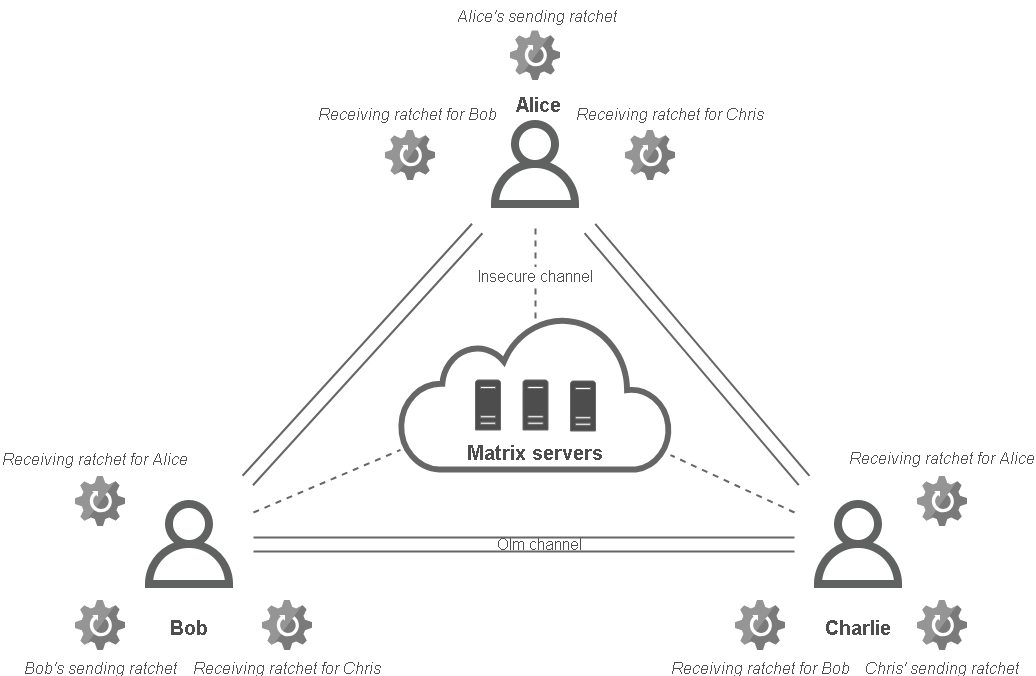
\includegraphics[width=14cm]{figures/megolm_conceptual.png}
	\caption{Conceptual model of Megolm with three participants.}
	\label{fig:megolm}
\end{figure}

When a session is started a sender will send his initial ratchet key to each recipient, so that the sender ratchet and each recipients ratchet are in sync. This key exchange happens over a secure communication channel (Olm). Furthermore there is send N-1 initial messages when a session is initiated. Until a new session is started no further session keys are exchanged and the corresponding message keys are generated by incrementing the ratchet.

When a sender sends a message a message key is generated from the ratchet key and the message is encrypted using that message key. The message will be signed so the recipient will know which sender the message is from and which ratchet to utilize. %(not with a long-term I guess? hence providing deniability)
The message  is then send to the server which relays the message to all recipients over an insecure channel. When they receive the message the same message key is generated using the corresponding receiver ratchet and the message is decrypted. 

When a new participant joins the latest ratchet key would then be shared by each participant over Olm (or an earlier one if he should have access to historical conversation). 

When a participant leaves a new session would be initiated yielding in refreshing the ratchet keys hence not making it possible for that ex-participant to decrypt any further messages.




% add figures for naive olm and multicast encryption solution

The Matrix Protocol will be evaluated in the context of Megolm. The evaluation of the Matrix protocol heavily relies on the security assessment by NCC.


\subsubsection{Evaluation}

The Matrix Protocol provides several security properties shown in the table xx. 

It is worth mentioning that there is a trade-off between security and usability which must be decided at application layer. The most secure configuration would come at the cost of usability and performance.    
\begin{itemize}
	\item \emph{Usability}. From a users point of view it would be nice to have the possibility to load historical conversation instead of having to keep full history locally. Matrix supports multiple devices and if a participant adds another device at some later point it makes sense to load the participants historical conversation into the device. From a security perspective this would mean that the \emph{initial ratchet state} is stored and is send to the new device so every message key can be generated. This certainly goes against the principle of forward secrecy. The most secure configuration would not store the \emph{initial ratchet state} hence satisfy forward secrecy thus disable the described usability feature \cite{ncc} \cite{megolm}.
	\item \emph{Performance}. When a megolm session is initialized there is an initial burst of messages to exchange the initial ratchet key which is then stored in a \emph{initial ratchet state} value at each recipient. If this key is compromised then any future key can be generated for that session. To satisfy backward secrecy this would mean initiating a new session for each message which would trigger a burst of messages to exchange the ratchet key \cite{ncc} \cite{megolm}. This would scale poorly for a large group or when sending large-sized messages. 
\end{itemize} 


\begin{figure}[H]
	\hspace*{-1.7cm} 
	\centering
	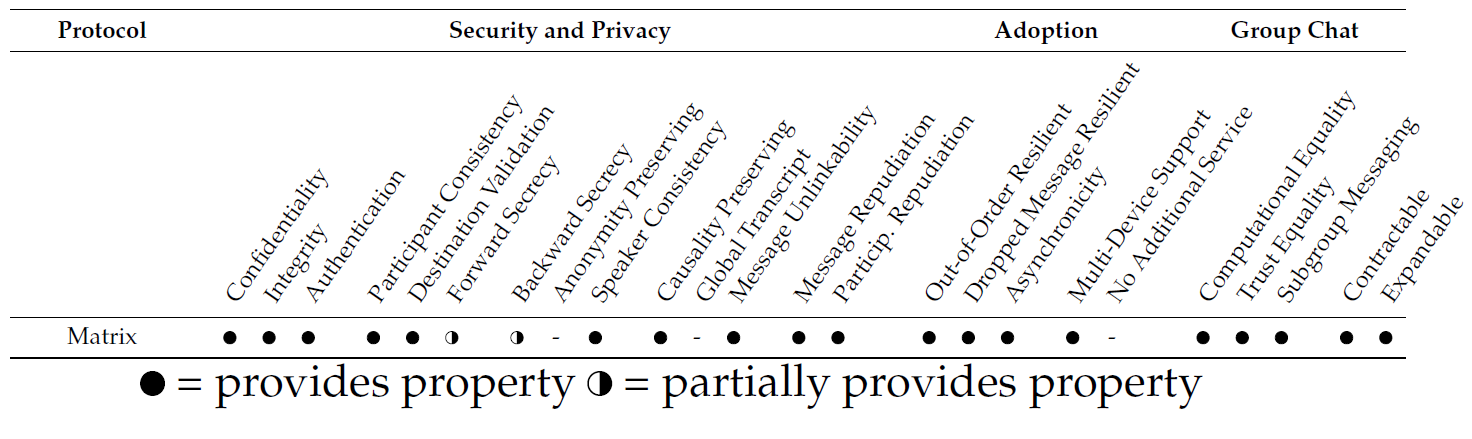
\includegraphics[width=16cm]{figures/framework.png}
	\caption{Evaluation of Matrix Security.}
	\label{fig:framework}
\end{figure}

Some of the security properties in the table are briefly examined.

\subparagraph{Confidentiality} When a message is send it is encrypted and can only be decrypted by the intended recipients who has the corresponding ratchet session key received over an Olm channel. 

\subparagraph{Integrity} The receiver will only accept a message if it is successfully decrypted hence if in transit a message was modified then the message would be rejected. 


\subparagraph{Forward secrecy} Each participant keeps a \emph{initial ratchet state} which holds the earliest ratchet session key for a session. This clearly violates forward secrecy since every message can be decrypted if the \emph{initial ratchet state} value is compromised. However it is a deliberate trade-off for usability to enable historical conversation and storing the value is optional. Since this is an optional feature the forward secrecy is partially provided \cite{ncc}. 

%From NCC

\subparagraph{Backward secrecy} If a ratchet key is compromised then an adversary can generate every message key from that point on hence intercept any message that sender sends to the group. This can be prevented strictly by starting a new session with every send message however it would not be possible to keep conversation history (only locally when data is encrypted). Hence the property is only partially provided \cite{ncc}.

% From NCC


\subparagraph{Speaker consistency}

There is no guarantee for speaker consistency. A well known problem of multi-cast encryption group chat is transcript inconsistency. A sender may send different messages to different recipients. However it requires that the server is in collusion with the sender. This also applies to \emph{\textbf{Causality preserving}} \cite{ncc}.


\paragraph{Other properties}

The multi-cast encryption design does not provide \emph{participant consistency} \cite{sok}.

The properties \emph{Dropped message resilence} and \emph{Out-of-order resilient} are provided by keeping track of ratchet indices. 

Several properties are inherited from the secure key exchanging channel provided by Olm while other properties are inherited because of asynchronicity of the Megolm protocol.

\begin{itemize}
	
	\item \emph{Authentication} is provided by Olm since the ratchet session key is send to the recipient through an Olm channel or else the message key could not be derived.
	\item \emph{Destination validation}. The ratchet session key is exchanged over a secure Olm channel hence only the intended recipient could decrypt it.
	\item \emph{Anonymity preserving} is not provided since Olm requires the long-term public key in the initial key exchange.
	\item \emph{Global transcript} is also not provided because of the asynchronous nature of the Megolm protocol.  
	\item \emph{Asynchronicity} is obviously provided.
	\item \emph{Deniability} properties are inherited from Olm as well.
\end{itemize}

All properties related to group chat are also provided. Although they are additional features and not related to security. 


\paragraph{Other findings}

\subparagraph{Message Replays}

Matrix allows decryption of a message multiple times hence it is vulnerable to replay attacks. Replay attacks are handled at the application layer. Whenever a message is decrypted a message index is generated and stored. If the exact message is decrypted again the same message index will be generated and can be compared to the stored message index making the replayed message invalid. 

\subparagraph{Unknown key-share attack}

The \emph{Unknown key-share attack}\footnote{https://en.wikipedia.org/wiki/Unknown\_key-share\_attack} is a vulnerability found with a high risk in Megolm. The vulnerability is inherited from Olm and occurs after the initial message in Triple-DH. 

The vulnerability has been mitigated at the application layer by providing a unique identifier for the sender and receiver into each message and then checking the values when decrypted \cite{ncc}.

\paragraph{Recent research}
The way backward secrecy would be provided in Matrix is computationally expensive. Recent research has proposed solutions with early implementations for these problems with IETF leading the research on the standard on \emph{Messaging Layer Security}. Matrix has expressed awareness of the protocol and a possibility of adaption in the future.

\subsection{End-to-end security} \label{endtoend}

Section xx describes Matrix long-term goal as being a generic HTTP messaging API. It could be utilized for any kind of data exchange in a system or between multiple systems.

A system using the Matrix Protocol for exchanging data would benefit from the security properties found in the evaluation yet the system-wide security or end-to-end security would be incomplete an further measures must be taken. Such system might demand confidentiality and integrity throughout the system yet the system as a whole would have a different threat model than the one described for a secure messaging system hence no guarantee of confidentiality or integrity beyond the endpoints in end-to-end encryption. 

The following figure depicts how end-to-end encryption might be inadequate in such system. 

\begin{figure}[H]
	\centering
	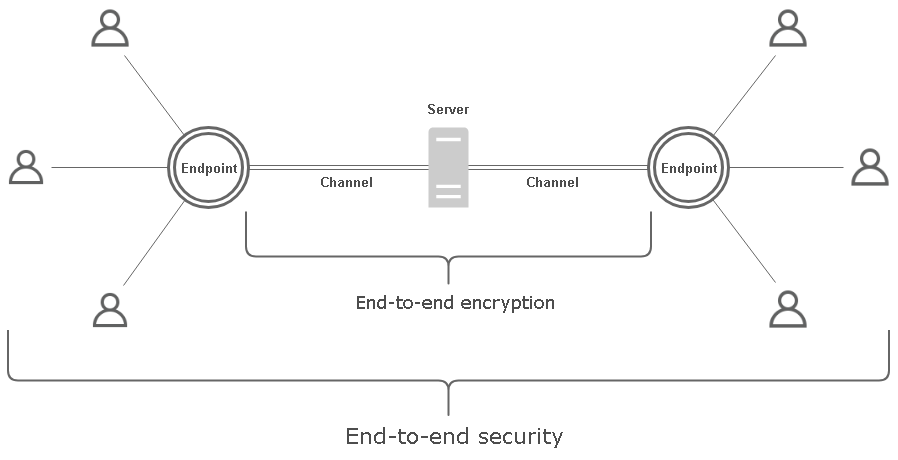
\includegraphics[width=12cm]{figures/e2esecurity.png}
	\caption{End-to-end security.}
	\label{fig:e2esecurity}
\end{figure}

As the system depicts there might be several principals accessing the endpoint. Each principal could retrieve some information possibly protected with access control. Assume that the information resting at the endpoint is of confidential nature; access could still be granted with no respect of the confidentially of that information. There clearly lack a mechanism of specifying what information is confidential or public and where it may flow under what conditions.  

\subparagraph{Matrix IoT}
Matrix identifies IoT as another use case. A person can have several devices for health tracking, entertainment and so on. The data from the devices are send to vendors - a device might send data to several vendors. Ultimately this give a fragmentation of the person's own data with it being placed at several vendors data back-end. Matrix proposes a solution where all the device data for a person is synchronized and persisted on Matrix. Vendors would be connected to Matrix. This is depicted in figure \ref{fig:matrix_iot} below. 

\begin{figure}[H]
	\centering
	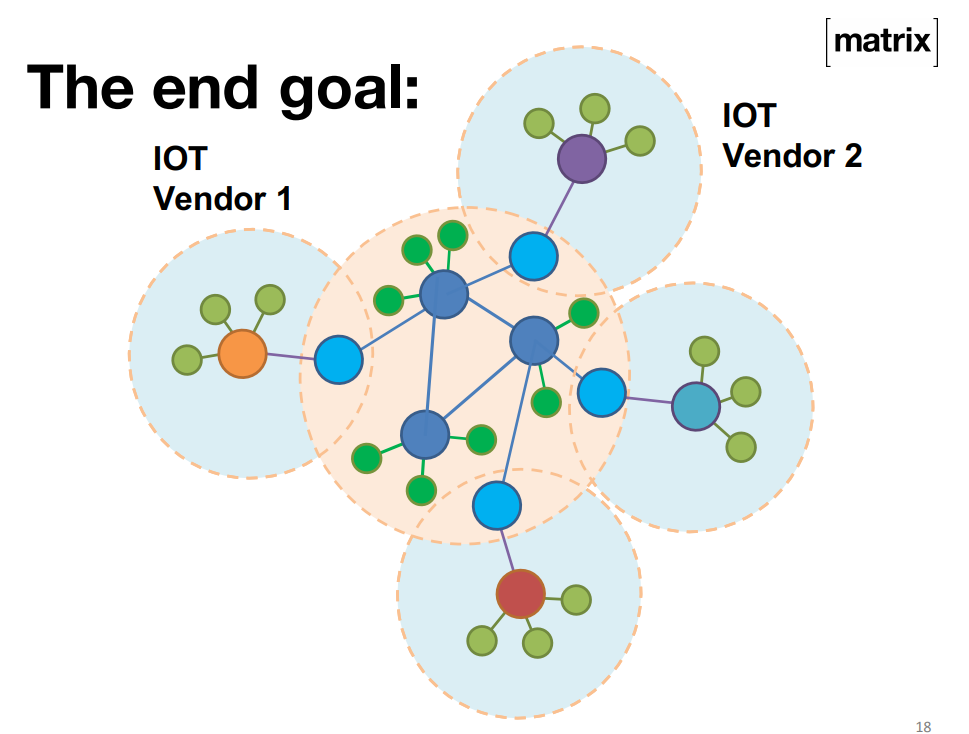
\includegraphics[width=10cm]{figures/matrix_iot.png}
	\caption{End goal for Matrix IoT}
	\label{fig:matrix_iot}
\end{figure}

The data flowing from the sensors to Matrix might be of sensitive nature or the owner might only allow some data to flow to some vendors under specific conditions. This issue related to confidentiality is not addressed by Matrix. 

\subsection{Evaluation summary}

In this section an evaluation of Matrix security was presented. Several security properties are a part of Matrix security model with forward secrecy and backward secrecy being provided depending on the Matrix configuration.

End-to-end encryption is not the end of security. Other security measures must be taken to provide confidentiality and integrity. Information Flow Control is such measure and the next section will present a survey on Information Flow Control.




\chapter{Survey of Information-Flow Control Tools} \label{surveychapter}


\section{Information Flow Control} %mere konkret og teknisk
%Selvom jeg ikke kiggr på fx trafic analysis så er det vigtigt at nævne og påpege det ikkeer noget jeg løser
In the beginning of this chapter, the security properties confidentiality and integrity were mentioned which are major security goals for a system. If there is \emph{secure information flow} throughout the system, then confidentiality and integrity is achieved \cite{Hedin2011}. Secure information flow means that only authorized flow of information is allowed \cite{Denning1976}. There are two aspects to secure information flow; the reading of the information (confidentiality) and the writing of the information (integrity) \cite{Hedin2011}. 

\emph{Information Flow Control} is a \emph{security mechanism}\footnote{"A security mechanism is a method, tool, or procedure for enforcing a security policy" \cite{Bishop2004}} for achieving secure information flow.
Information Flow Control is a language-based security technique that can enforce defined \emph{security policies}\footnote{"A security policy is a statement of what is, and what is not, allowed." \cite{Bishop2004}} concerning confidentiality and integrity of data. It enables us to express where information may flow to and under what conditions. 

\subsection{Lattice model}\label{lattice}

By classifying information with \emph{security levels}, we can express where information may flow. Consider the following confidentiality policy; we classify \emph{secret} as secret information, and classify \emph{public} as public information. For the two security levels we express what information may flow where by classifying information with a security level, It holds that flow from public to public is allowed, public to secret is allowed, and secret to secret is allowed. For preserving confidentiality, flow from secret to public is under no circumstances allowed.  This can be expressed as \emph{public $\leq$ secret}, and we can formalize these flow constrains by means of a lattice\footnote{https://en.wikipedia.org/wiki/Lattice\_(order)} structure where information flows upwards shown in figure \ref{fig:lattice}a \cite{Smith}.


\begin{figure}[H]
	\centering
	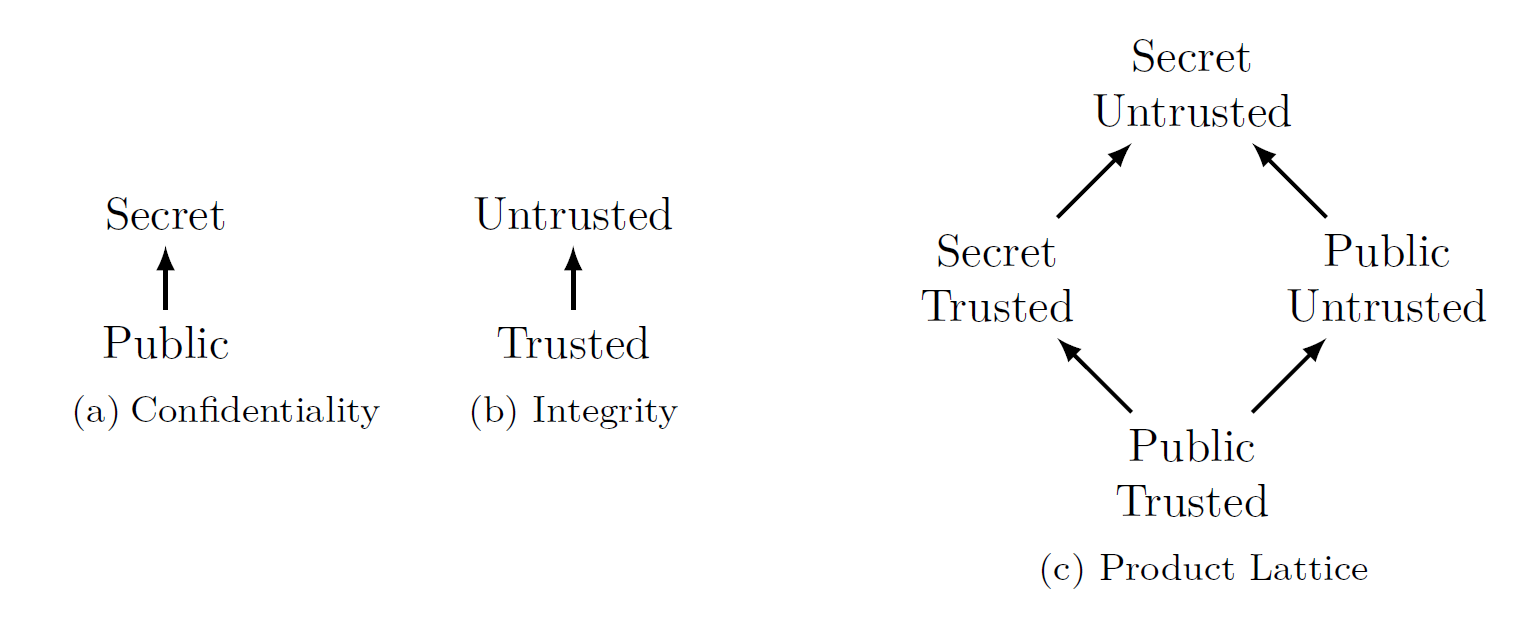
\includegraphics[width=12cm]{figures/lattice.png}
	\caption{ Lattice model for confidentiality and integrity \cite{Musard2014}}
	\label{fig:lattice}
\end{figure}

Likewise, a policy for integrity can be specified where information from an \emph{untrusted} source must not flow to information with a security level of \emph{trusted}, which is exactly the opposite of the confidentiality policy. Figure \ref{fig:lattice}b illustrates an integrity lattice. By combining the two we get a lattice show in figure \ref{fig:lattice}c.

\subsection{Explicit and implicit flow}\label{explicitimplicit}
The problem with mainstream programming languages is that they are unable to enforce defined policies such as the confidentiality and integrity policies described in the previous section. Consider the following flow:

\begin{lstlisting}
public = secret;
\end{lstlisting}

This is an \emph{explicit flow} since the \emph{secret} value is directly copied into the \emph{public} value, which obviously is a violation of the confidentiality policy and is an insecure flow of information \cite{Hedin2011}. 

Another example of insecure information flow is \emph{implicit flow}:

\begin{lstlisting}[language=ALGOL]
public = false;
if secret then public = true
\end{lstlisting}

In this example, the \emph{secret} value affects the control flow and some information is leaked about the \emph{secret} value. Hence this also violates the confidentiality policy. When secret values can affect the control flow there is an implicit flow \cite{Sabelfeld2003}.
%Security is equivalent to \emph{secure information flow}

\subsection{Covert channels} The explicit and implicit flows can also be considered as \emph{channels} that signal information \cite{Kashyap2011} \cite{Sabelfeld2003}. \emph{Covert channels} are channels that are not meant to signal information but somehow leaks information \cite{Kashyap2011}. The most prominent covert channels are: 
\begin{itemize}
	\item \emph{Implicit channels} leaks information through the path the program takes in the control flow.
	\item \emph{Termination channels} leaks information by considering if a program terminates.
	\item \emph{Timing channels} leaks information by considering when an action occurs or how much time a program takes.
\end{itemize}

Other channel are \emph{probabilistic channels}, \emph{resource exhaustion channels}, and \emph{power channels}. It is not necessarily all covert channels that are of concern and in the end depends on what is observable by an adversary \cite{Sabelfeld2003}.

\subsection{Noninterference}
Secure information flow can be expressed by the concept of \emph{noninterference}. The notion of noninterference is that someone observing the public input and output of a system and can pick the public input should not be able to learn anything about the secret input of the system. If the secret input interferes with the public output then there is information leak. The figure \ref{fig:noninterference} illustrates noninterference \cite{Hedin2011}.  

% The policies defined in section \ref{lattice} are noninterference policies \cite{Sabelfeld2003}. 


\begin{figure}[H]
	\centering
	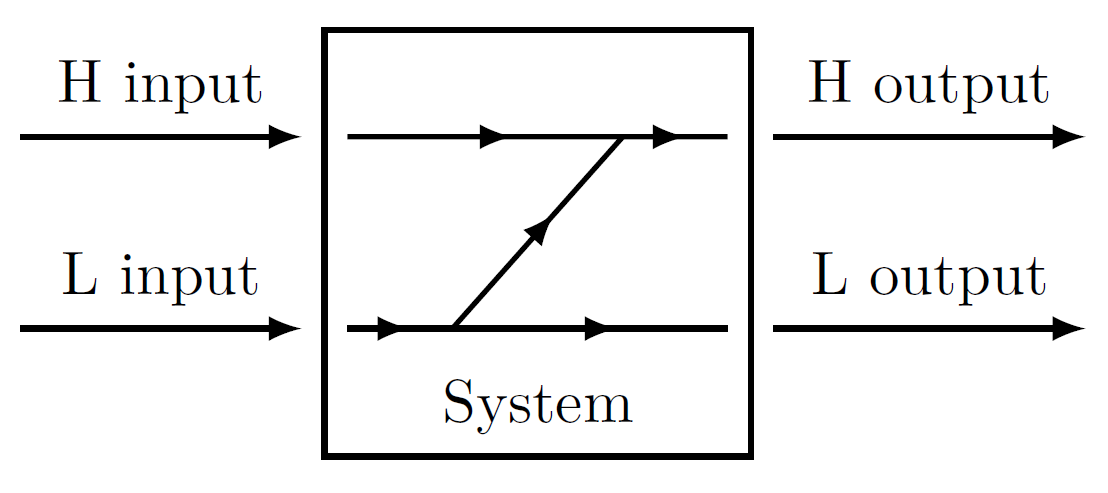
\includegraphics[width=8cm]{figures/noninterference2.png}
	\caption{ Noninterference \cite{Musard2014}}
	\label{fig:noninterference}
\end{figure}

The figure illustrates that the low confidentiality output \emph{L} (public) should be independent of the \emph{H input} (secret). In other words if a program is executed with fixed public input but with different secret input; then there should not be any changes to the public output \cite{Hedin2011}.


Depending on what an observer is capable of observing; different variations of noninterference can be expressed. Two of such variants are \emph{termination-insensitive} and \emph{termination-sensitive}.


\subparagraph{Termination-insensitive noninterference}

Termination-insensitive noninterference would guarantee that when a program terminates; the program's public output remains unaffected of the secret input. However it is possible to leak information through termination channels. By observing termination; 1 bit leaks can be achieved for each run of the program \cite{Hedin2011}:

\begin{lstlisting}
if (secret == public) then while (true) do skip done
\end{lstlisting}

If the program does terminate then the observer has learned that the secret is not equal to the public value hence 1 bit of information is leaked. 

%Save the argument of more than 1 bit leak to the discussion.

\subparagraph{Termination-sensitive noninterference}
The alternative is the termination-sensitive noninterference variant. The public output is independent of the secret input. Furthermore if the program is run with secret input \emph{s\textsubscript{1}} and it terminates; then the program run with secret input \emph{s\textsubscript{2}} would terminate as well. Hence if \emph{s\textsubscript{1}} did not terminate then \emph{s\textsubscript{2}} would not either \cite{Hedin2011}.

This variant of noninterference does not allow secret variables as guards in loops  and if-else-than statements as long as those in no way affect possible future \emph{L} output. This variant would be more restrictive and disallow flows as such \cite{Hedin2011}:

\begin{lstlisting}
while (secret == true) do ... done
\end{lstlisting}

\subsection{Declassification}
Noninterference is a very strict policy and not practical. Consider the classic example of a user logging into a system. It is unavoidable that a login attempt gives some information away about whether or not the password combination was valid. If the password is incorrect the login fails and partial information is given away. There is no problem with the above and is regarded as secure. Another example is sending encrypted data over an insecure channel; secret input is encrypted and the cipher text would then be sent over an insecure channel. However this goes against noninterference since the secret input clearly interferes with public output \cite{Hedin2011}.

Declassifying of information is necessary. Taking some specific information from a higher security class and changing it to a lower security classification is declassification. When declassifying information the following four dimensions needs to be addressed \cite{Sabelfeld2009}:

\begin{itemize}
	\item \emph{What} information should be declassified. We would like to specify what information is released.
	\item \emph{Who} can declassify the information. By specifying exactly who can release information it rules out that someone unspecified can make unintended leaks through declassification.
	\item \emph{Where} the information can flow. The dimension describes which security levels the declassified information may flow to and also where in the code the declassification occurs. 
	\item \emph{When} the declassification occurs. The release of information is only allowed relative to some even e.g. only after a purchase can a software key be released.
\end{itemize}



\subsubsection{Decentralized label model}\label{dlm}
\emph{Decentralized Label Model} allows us to define flow policies and address declassification of information in a program. A policy is defined by adding \emph{labels} to a value. A value can hold information for different \emph{principals} called \emph{owners}. A label \emph{L} specifies an \emph{owners} set \emph{owners(L)}. Each owner can allow a list of principals called readers \emph{readers(L,O)} that the information may be released to. \emph{Effective readers} are readers that all owners agree on the information can be released to and is essentially those where information can flow to. An example of a label is \textbf{\{\emph{o\textsubscript{1}}:\emph{r\textsubscript{1},r\textsubscript{2}}; \emph{o\textsubscript{2}}:\emph{r\textsubscript{2},r\textsubscript{3}}\}}; where  \emph{o\textsubscript{1}} and \emph{o\textsubscript{2}} are the different owners with their specified readers \cite{Myers1997}. The example \emph{L} has the following:

\[owners(L) = \{o_1, o_2\}\]
\[readers(L,o_1) = \{r_1, r_2\} \]
\[readers(L,o_2) = \{r_2, r_3\} \]
\[effectiveReaders(L) = \{r_2\} \]

Such labeling makes it possible for each owner to have an independent flow policy and give control of where the information may flow. Declassification is possible if the program detects it is running as the authority of one of the owners \cite{Myers1997} \cite{Myers1998}. This is known as the \emph{principal hierarchy} and can allow a principal to act for another principal.

%Apart from labels, there is one other important component to the DLM, namely the principal hierarchy, specified by a reflexive and transitive acts-for relationship. If Eve acts for Dave then Eve can do anything that Dave can. In the example above this means Eve can also read data with the label given above.

\subsection{Information-flow enforcement}
There exist two general techniques for enforcing secure information flow; \emph{static analysis} through e.g a type system, and \emph{dynamic analysis} through e.g. a monitor. Both techniques give the assurance of termination-insensitive noninterference \cite{Sabelfeld2010}. The static analysis have the advantage that it does not have the runtime overhead as the dynamic analysis while the dynamic analysis is more permissive \cite{Sabelfeld2010}. 


\subsubsection{Static enforcement}
Enforcement of information-flow through static analysis is done using type systems.
A simple type system is presented and shown in figure \ref{fig:typesystem}. 

\begin{figure}[H]
	\centering
	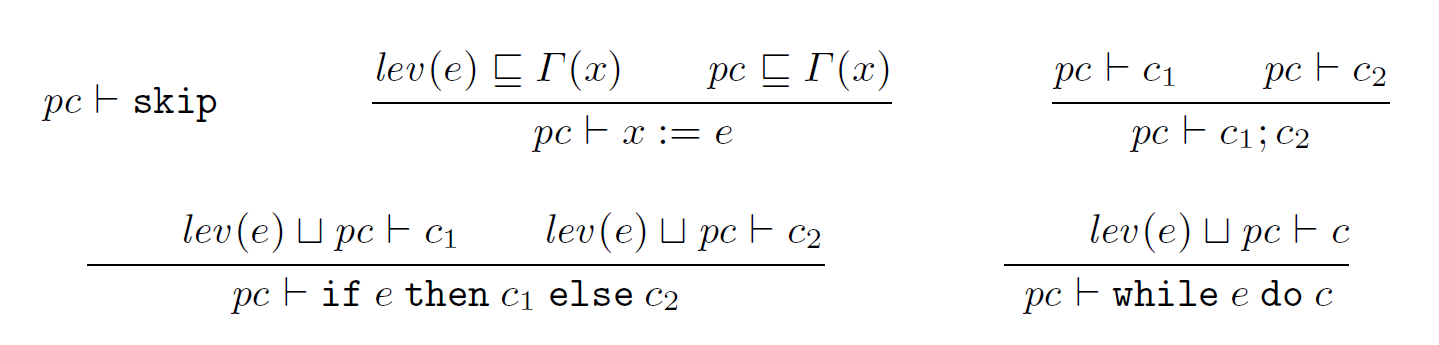
\includegraphics[width=12cm]{figures/securitytypesystem.png}
	\caption{ Typing rules \cite{Sabelfeld2010}}
	\label{fig:typesystem}
\end{figure}

We assume that the security lattice has the levels \emph{L} for low (public) and \emph{H} for high (secret). $\Gamma$ denotes a typing environment that takes a variable \emph{x} and maps it to a security level. The function \emph{lev(e)} takes an expression \emph{e} and returns a security level; if \emph{e} holds a high variable then \emph{H} is returned or else \emph{L} is returned. The security level of the context is kept tracked of by the program counter \emph{pc}. The typing judgment for commands is denoted by \emph{pc $\vdash$ c} \cite{Sabelfeld2010}.

The typing rule \emph{pc $\vdash$ x := e} is for assignment; it prevent assignment of a expression that holds a high variable to a low variable \cite{Sabelfeld2010}. Hence the explicit flow would be detected by the type system:

\begin{lstlisting}
low = high
\end{lstlisting}

Furthermore implicit flow are detectable through the program counter \emph{pc}. If there is a high guard then the \emph{pc} has the security level \emph{H} and would expect assignments of high variables hence preventing low assignments \cite{Sabelfeld2010}. The implicit flow would be detected by the typing system as well:

\begin{lstlisting}
if high then low = true else low = false
\end{lstlisting}


\subsubsection{Dynamic enforcement}
Dynamic analysis is provided with \emph{monitors}. Monitoring can only consider one path when running. This has led to the belief that the dynamic approach falls short compared to the static enforcement. However both dynamic enforcement and static enforcement achieve termination-insensitive noninterference hence they give the same security assurance \cite{Sabelfeld2010}. 

\begin{figure}[H]
	\centering
	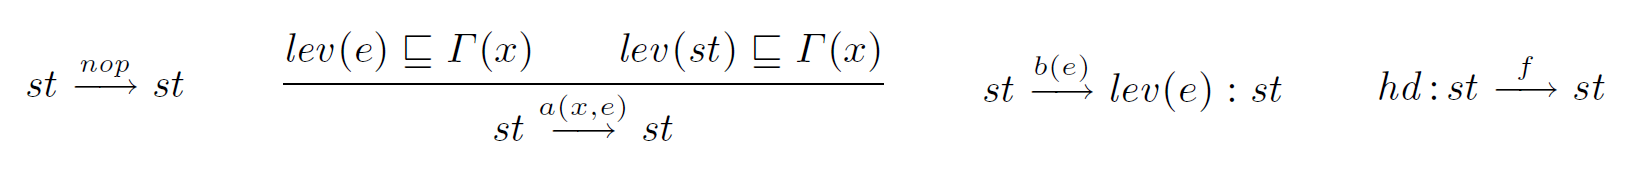
\includegraphics[width=12cm]{figures/monitoringrules.png}
	\caption{ Monitoring rules \cite{Sabelfeld2010}}
	\label{fig:monitoring}
\end{figure}

The figure \ref{fig:monitoring} shows monitoring rules for a monitor. Programs generates events and the monitor chooses to accept an event or block it by halting. Security levels are tracked by stack \emph{st} which is called a \emph{monitor configuration} and serves the same purpose as the program counter; keeping track of the current security context.  The monitor can execute following \emph{events} generated by the program: 

\begin{itemize}
	\item \emph{nop event:} signals a skip and the monitor always this event. It does not change the state of the monitor.
	\item \emph{assignment event a(x,e):} assigns the value of expression \emph{e} to variable \emph{x}. It does not change the state of the monitor but the monitor has the following two conditions:
	\begin{enumerate}
		\item \emph{lev}(\emph{e}) $\sqsubseteq$ $\Gamma(x)$: the expression \emph{e}'s security level is equal or lower than variable \emph{x}'s security level.
		\item \emph{lev}(\emph{st}) $\sqsubseteq$ $\Gamma(x)$: the highest security level in the stack is equal or lower than variable \emph{x}'s security level 
	\end{enumerate} 
	\item \emph{branching event b(e)}: branches on \emph{e} and changes the state of the monitor. The security level of \emph{e} is pushed on the stack.
	\item \emph{event f}: signals are loop or if-else statement has finished evaluating. The security level pushed to the stack \emph{st} would be popped when evaluation is finished.
\end{itemize}

The first condition for the assignment event prevents explicit flows, since whenever the program takes a step, the monitor must take a step; if the monitor cannot take a step, that halts the program. The second condition prevents implicit flows as such: 

\begin{lstlisting}
if high then low=true else low=false
\end{lstlisting}

The mechanism related to the branching event aids in preventing implicit flows by pushing the security level of \emph{st} to the stack. Now consider the following code: 

\begin{lstlisting}
if high then low=true else skip
\end{lstlisting}

If high is \emph{false} then the code would continue however if high is \emph{true} the execution would be stopped. Hence 1 bit would be leaked and is acceptable in context of termination-insensitive noninterference.

\section{Summary}
The background section introduces security properties necessary for a secure system. Several other security properties are described relevant for a secure messaging system which is relevant for the section \ref{evaluationofmatrix} where Matrix security is evaluated. This section also presented a description of the Signal Protocol necessary for the evaluation as well. Furthermore Matrix and its architecture was described and finally the basic concepts of Information-Flow Control was presented.


\section{Analysis of IFC Tools}
%Enforcing new session start every time a patient journal is sent. Could it be enforced with IFC?
% Tools issue: java sdk for matrix is beta and not fully implemented. 
% Best supported sdk is for javascript or python. Problem of running javascript code or python code with Paragon (java)
% Maybe better to use JSFlow instead 

% This chapter will present the criteria \emph{Survey of IFC tools and selection of tool}


Different Information-Flow Control tools were considered to be used in the case study. This section describes three of those tools; \emph{Jif}, \emph{Paragon} and \emph{JSFlow}. This section further justifies the selection of Paragon.

\subsection{Jif}

Jif is a Java based security-typed programming language that provides information flow control through static enforcement. Jif implements the Decentralized Label Model (DLM) described in section \ref{dlm}. Policies are defined conforming to the DLM. The policies are enforced at compile time by and Information-Flow Security type system with support for enforcement of dynamic policies at runtime. If a Jif program adheres to the specified policies the Jif compiler then compiles it to a secure Java program \cite{jifmanual}. 

Each variable in Jif has a DLM
policy associated with it. A policy
is
A policy is defined by labels and are associated with program variables. A policy can specify multiple principles that have readers or writers. A policy is defined as: 

\begin{lstlisting}[mathescape]
int {Alice$\rightarrow$Bob; Alice$\leftarrow$Bob} x;
\end{lstlisting}

The policy specifies two things; that first part with "$\rightarrow$" expresses \emph{Alice} controls the variable x and the variable can be read by \emph{Bob}, the second part with "$\leftarrow$ expresses that bob can write to it \cite{jifmanual}. 

The following code shows another example:

\begin{lstlisting}[mathescape]
int {Alice} x;
int {Alice$\rightarrow$Bob} y;
x = y; // OK
y = x; // BAD
\end{lstlisting}


Variable  \emph{x} has a policy that \emph{Alice} controls with no readers. The variable \emph{y} is owned by \emph{Alice} with \emph{Bob} being able to read hence the label is less restrictive than \emph{x}'s label. The compiler allows the \emph{x = y} since \emph{Bob} is specified as a reader for \emph{x}. However the expression \emph{y = x} is illegal since \emph{x} has a stronger policy than y and the explicit flow is caught \cite{jifmanual}.


A important feature for security-typed languages are declassification. Noninterference is too strict for practical programs thus it is necessary to declassify information at times. The following example has two variables with different labels. Variable \emph{x} is more restrictive than \emph{y}; that has \emph{Bob} as a reader. The example depicts an implicit flow: 

\begin{lstlisting}[mathescape]
void implicitFlow(){
int {Alice$\rightarrow$} x;
int {Alice$\rightarrow$Bob} y;
if (x == 1) { 
// pc has label {Alice$\rightarrow$}
y = 0; // BAD
}
}
\end{lstlisting}

When the code branches on the if statement the pc has the label \emph{\{Alice$\rightarrow$\}} and the expression \emph{y = 0} becomes illegal since it has the label \emph{\{Alice$\rightarrow$Bob\}} which is less restrictive than the label pc is holding. If for some reason we would want the expression to become valid we would have to declassify it:

\begin{lstlisting}[mathescape]
void declassificationExample() where authority(Alice) {
int{Alice$\rightarrow$} x;
int{Alice$\rightarrow$Bob} y;
// PC has label {}
if (x == 1) {
// PC has label {Alice$\rightarrow$}
declassify({Alice$\rightarrow$} to {Alice$\rightarrow$Bob}) {
y = 0; // OK
}
}
}
\end{lstlisting}

To be able to declassify it must be through the authority of the owner. This has to be specified at the method definition. When the code branches on the if statement the program counter \emph{pc} has the label \emph{\{Alice$\rightarrow$\}} which can then be declassified to a label as restrictive as \emph{y}'s label \cite{jifmanual} \cite{Srikant}.

Another interesting feature is dynamic labels. Jif provides a run-time library which compares labels at runtime using a syntax that resembles if-statements.
\begin{lstlisting}[mathescape]
void m(int{*lbl} i, label{} lbl) {
int{Alice$\rightarrow$} x;
if (lbl <= new label {Alice$\rightarrow$}) {
x = i; // OK, since {*lbl} <= {Alice$\rightarrow$}
}
else {
x = 0;
}
}
\end{lstlisting}

The parameter variable \emph{i} has the label held by the label \emph{lbl} which would be resolved at runtime. Since the variable \emph{x} has label \emph{\{Alice$\rightarrow$\}}, we can allow a flow to that variable as long it is less or equally restrictive. The static analysis of the program will pass and the program will be able to compile.  
%Dynamic label example


Other relevant features that Jif supports are label inference\footnote{http://www.cs.cornell.edu/jif/doc/jif-3.3.0/language.html\#inference} and parameterized classes\footnote{http://www.cs.cornell.edu/jif/doc/jif-3.3.0/language.html\#parameterized-classes}.
\subsection{Paragon}

Paragon is a programming language that extends Java with the ability to express security policies for data. Paragon has similar characteristics to Jif and essentially solving the same problem. Paragon takes a different approach to defining information flow policies; \emph{Paralocks} \cite{paralocks} \cite{paragonpaper}.
At the core, \emph{Paralocks} is based on the concepts \emph{actors} and \emph{locks} \cite{paralocks}. An actor is a user with some role. For information can flow to an actor there might be a condition that states; that the actor must be of a specific role. These conditions are represented by boolean variables \emph{locks} and can be modified throughout program execution. These locks are called \emph{parameterized locks} since they are parameterized over actors. Policies are specified by parameterized locks and \emph{actor polymorphism} allows us to reason about all actors \cite{paragonpaper}.


In Paragon policies are immutable and the following example shows how policies can be defined:

\begin{lstlisting}
public static final policy low  = { Object x: };
public static final policy high = { };
\end{lstlisting}

Policies for \emph{low} and \emph{high} can encoded in different ways. The encoding specifies the most liberal policy that anyone can see the data that has the policy of \emph{low}. The actor is any \emph{Object x} hence anyone can read. The encoding for \emph{high} is the most strict policy and specifies that actors so no one can see the data \cite{paragonprogramming}.

To support a simple declassification mechanism a lock would have to be introduced and the \emph{high} policy definition would have to be redefined:

\begin{lstlisting}
private lock Declassify;
public static final policy low  = { Object x: };
public static final policy high = { Object x: Declassify};
\end{lstlisting} 

The \emph{high} policy now specifies that information can only be read if the \emph{ declassify lock} is open. The following method can now allow declassification:

\begin{lstlisting}
public static ?low int declassify(?high int x){
open Declassify { return x; } 
}
\end{lstlisting} 

The method is a custom declassification method for variables with type \emph{int}. By using Java generics the same method could be used for any type. The \emph{declassify()} method takes a parameter that has the policy \emph{high} and returns the parameter with the lower policy \emph{low}. The method opens the lock hence allowing the value of \emph{x} to be read and returned. 
%Java generics is used to allow declassification of any type.

\begin{lstlisting}
publicVariable = declassify(secretVariable); // OK
\end{lstlisting} 


The example illustrates a simple declassify method however it can be called by anyone. To ensure that only those with the right authority can call it the example could easily be extended with another lock \cite{paralocks}. 

It is possible to support policies at runtime with locks \cite{paragonprogramming}. Suppose we have a customer who buys some software. The software keys should only be given when the customer has paid. We define the following:

\begin{lstlisting}
public static lock Paid;
?{customer: } String customerData
?{customer: Paid} String softwareKey
\end{lstlisting}

When the the customer's payment is processed the lock \emph{Paid} should only be open if the payment is successful. 

\begin{lstlisting}
public void processPayment() {
// customer pays for item
if (paymentSuccessful) { open Paid; } else { ... }
}
\end{lstlisting}

It is not possible for the compiler to learn the state of the lock \emph{Paid}. By using the lock in a conditional statement the lock will be checked at runtime \cite{paragonprogramming}.

\begin{lstlisting}
processPayment();
if (Paid) { customerData = softwareKey; } else { ... }
\end{lstlisting}   

Paragon is a powerful tool for Information-Flow Control and has an interesting policy language with support for expressive dynamic policies. Other relevant features in paragon are policy inference and Java generics.

\subsection{JSFlow}

JSFlow is a tool for tracking information flow in JavaScript web applications. This tool is not a programming language as the two previously described tool but a JavaScript interpreter that supports full non-strict ECMA-262 \cite{jsflowsite}. JSFlow enforces secure information flow through dynamic analysis and can detect explicit and implicit flows. JSFlow uses a program counter \emph{pc} to track the security context. JSFlow defines two built-in security levels; \emph{public} and \emph{secret}, it also supports custom security labels on values. JSFlow allows pure explicit flows by upgrading the security label of the variable being assigned to \cite{jsflowsite}:

\begin{lstlisting}
high = lbl(true);
low = high;
\end{lstlisting}

The variable \emph{high} is assigned a secret value denoted by the \emph{lbl} function. When \emph{high} is assigned to \emph{low} the security label is upgraded for low. JSFlow prevents implicit flow through \emph{no sensitive update} that under secret control disallows changes to security labels \cite{Hedin2014}:

\begin{lstlisting}
high = lbl(true);
if(high){
l = true;
}
\end{lstlisting}

The execution would halt for the above code since no sensitive update is allowed. 

As mentioned before security labels can be assigned to variables. In the following examples \emph{l}, \emph{m} and \emph{h} is defined with different labels.

\begin{lstlisting}
var l = lbl(10, 'low');
var m = lbl(15, 'mid');
var h = lbl(20, 'mid', 'high');
if(m === 15) {
h=m; // OK
l=m; // BAD
}
\end{lstlisting}

JSFlows uses a subset lattice hence \emph{m} can flow to \emph{h} since \emph{m}'s label is a subset of \emph{h}'s labels \cite{jsflowsite}. The assignment \emph{l=h} would halt since the \emph{m}'s labels is not a subset of \emph{l}'s labels.


JSFlow is an exciting tool for dynamic Information-Flow Control. However the JSFlow is still immature and does not support important features such as declassification.

\subsection{Selection of IFC tool}
The approach to selecting a tool is from a programmer's perspective with emphasis on choosing the right tool for developing rather than the tool that achieves the best security. The rationale behind this is that if the tool is too strict, it is impossible to write practical programs in it.
The selection of the tool is based on different parameters that falls into two categories; \emph{technical features} and \emph{soft parameters}. The technical parameters are related to features that are necessary for developing the prototype while the soft parameters considers other aspects such as documentation, flexibility and permissiveness.

The technical features are relevant for applying the tool. The tool must have the following features; 

\begin{itemize}
	\item \emph{Define policies:} It must be possible to express where information may flow.
	\item \emph{Declassification:} Noninterference is too strict and the ability to declassify information is necessary. 
	\item \emph{Policy inference:} The tool can automatically infer labels to avoid retyping labels.
	\item \emph{Support for external libraries:} An important feature since the tool should be applicable to a Matrix SDK library.
	\item \emph{Run-time label checking} to enforce dynamic labeling.
\end{itemize}

The soft parameters are indirectly related to the tool. It can be an overhead developing if the program is to strict hence \emph{permissiveness} is defined as a parameter. The parameter \emph{flexibility} covers the flexibility and restrictiveness of the tool; it should be uncomplicated and straightforward work with the policy language. The final soft parameter is \emph{documentation}.

The table below gives an overview of the three tools related to the parameters. 

\begin{table}[H]
	\hspace*{-1.2cm} 
	\centering
	\begin{tabular}{r|ccccccccc}
		&
		\rot{Defining policies} &
		\rot{Declassification} &
		\rot{Run-time label checking} &
		\rot{Policy inference} &
		\rot{Support for external libraries} &
		\rot{Documentation} &
		\rot{Flexibility} &
		\rot{Permissiveness}
		\\ \hline
		Jif     & X & X & X & X & X & X &   &    \\ 
		Paragon & X & X & X & X & X &   & X &    \\
		JSFlow  & X &   & X & x &   &   &   & X  \\ 
	\end{tabular}
	
	\caption{Comparison of IFC tools}
	\label{fig:toolcomparison}
\end{table}


% Not possible to use Matrix library with JSFlow because of missing support for libaries such as require (in node). Also overhead with configuring JSFlow to be the interpretor.


JSFlow is still an immature tool and lack support important features. JSFlow does currently provide support for use with external libraries. It also lacks a mechanism for declassification. JSFlow would have been an interesting tool because of the permissiveness that comes with dynamic enforcement but also since the main Matrix SDK is for Javascript. 

Jif and Paragon offer many of the same features with the fundamental difference being the policy language. The policy language of Paragon is expressive, flexible and intuitive. Paragon is less restrictive and more flexible regarding the policies it specifies \cite{paragonpaper}. The programming experience in Paragon is more as an extension to Java then a different programming language which is the experience you get when programming in Jif. Jif however has a more complete documentation and more code examples to showcase. 

Another important aspect is the support for external libraries. Matrix can be used through client SDK's hence support for external libraries is necessary. Both Jif and Paragon supports this by allowing interacting with external Java classes. Both languages must specify a signature for the external Java class. %This was an overhead in Jif and even though Paragon uses the same approach it was easier to manage in Paragon.

Based on the consideration and parameters Paragon has been selected as the tool used in the case study. 


\section{Summary}
In this chapter the Matrix security model has been evaluated. Matrix provides end-to-end encryption and uses the Double Ratchet algorithm by Signal. To achieve end-to-end security the endpoints need to be secured as well \cite{Sabelfeld2003} this leads us to the chapter's second part. The chapter analyzed information-flow control tools and justifies the selection of Paragon which the prototype is programmed in. 

\chapter{Implementation}\label{implementation}

% This chapter presents the implementation of a distributed system running on Matrix and developed with Paragon as described in the criterias.

This chapter describes the implementation of the prototype. The prototype is a system for sending and retrieving patient journals among different hospitals. The system relies on Matrix as the secure communication channel and storage.


\section{Journal system}

% Describe the requirements for the journal system.
The journal system is inspired by the Danish E-journal system as described in section \ref{intro}. A journal system serves an important purpose by providing patient journals to different hospitals and clinics. If a patient arrives at the ER and the doctor cannot access the patient's journal then the treatment of the patient gets problematic. A doctor might miss out on important details about the patient or even worse prescribe medication that might give the patient an allergic reaction. The availability of a patient journal is a necessity however the number of medical employees that have access to such a journal has raised privacy concerns. Around 90.000 medical employees have access to patient journals. Consider the scenario where a patient gets referred to a physiotherapist with muscle pain. When the therapist opens the journal the full medical history will be present; if the patient had received psychiatric treatment those session would be readable too. Furthermore a patient journal is accessible by a large number of unrelated medical employees with the only prevention mechanism being logging and audit trails.


The lack of secure information flow is evident and the prototype demonstrates how Information-Flow control can be leveraged to enforce security policies concerning the information. The journal system is a small distributed system where Hospitals can send, receive and store patient journals. Matrix provides the distributed structure and is responsible for securely storing and transmitting the journals. Paragon provides secure information flow at the endpoints hence providing end-to-end security. 
The following requirements are defined for the prototype:

\begin{itemize}
	\item A patient journal contains low (public), medium (confidential) and high (secret)  information.
	\item A patient journal is send and received securely over a channel.
	%\item A patient journal can only be appended to. 
	\item Hospitals have shared access to patient journals. 
	\item A hospital has two actors: Doctor and Secretary.
	\item A secretary can only see low parts of the journal.
	\item A secretary can edit the public parts of a journal.
	\item A doctor can see the everything up to confidential information.
	\item A doctor must have the patient in care to gain the journal's secret information.
	\item A doctor can edit the public part and confidential parts of a patient journal.
	\item A doctor can only add to a secret fields in a patient journal if the patient has been referred to the doctor.
\end{itemize}

The following non-functional requirements are defined:

\begin{itemize}
	\item Confidentiality: the system must ensure the confidentiality throughout the system according to the security policies at all times.
	\item Integrity: the system must ensure that only intended actors can modify the specific parts of a patient journal.
\end{itemize}

The current journal systems allows medical employees to access the journals from anywhere. The prototype makes the assumption that the system can only be used within hospitals. Furthermore access for patients to their journal is not supported.

\subsection{System design} \label{systemdesign}

The system is distributed and allows to run multiple clients to send and retrieve patient journals. The system consists of two components; \emph{Matrix} and the \emph{client}. The Matrix component encapsulates the Matrix SDK and provides an interface to Paragon. The client component consumes that interface and can be considered as the endpoint in a communication channel. The client component provides secure information flow for data received through Matrix. Without the interface it would not be possible to achieve end-to-end security in the system. 
The component diagram in figure \ref{fig:matrix_component} depicts this.

\begin{figure}[H] 
	\hspace*{-1cm}
	\centering
	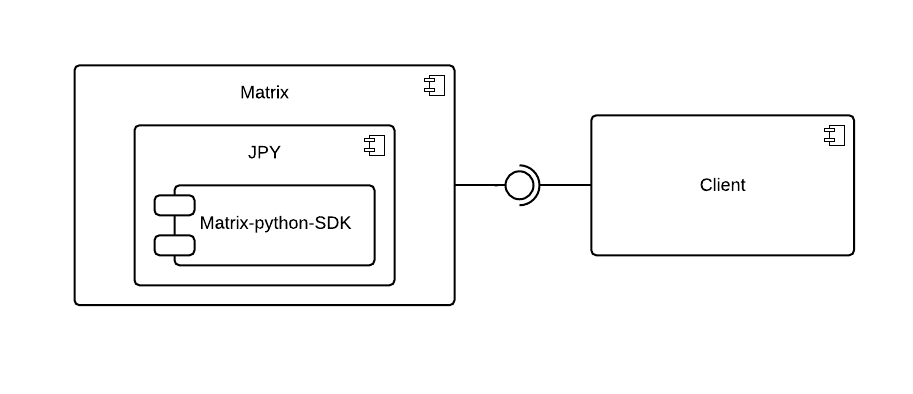
\includegraphics[width=14cm]{figures/matrix_component.png}
	\caption{Component diagram for the system}
	\label{fig:matrix_component}
\end{figure}

Matrix provides several SDK libraries that client application can be build on top of. The most prominent is the Javascript Matrix SDK. It is the best maintained with the largest feature set however it is not compatible with the Java based Information-Flow Control tool Paragon. A Java Matrix SDK exists but it is an early alpha version with end-to-end encryption not implemented yet. The Python Matrix SDK is another major SDK with support for end-to-end encryption in beta. The Python Matrix SDK is used in the Matrix component through a Java-Python bridge \emph{JPY} that can embed Python code in Java as shown in the Matrix component in figure \ref{fig:matrix_component} 




\subsubsection{Matrix}
%Matrix API's
% A lot of things are handled under the hood by the matrix SDK.
Matrix is an important component in the system. It manages the transmission and storage of patient journals through rooms while managing end-to-end encryption. The encryption mechanism is automatically provided and the SDK manages the session keys under the hood.  As described in section \ref{matrix:architecture} a room is a conceptual place for sending an receiving events and events can be any of any structure. The event history in a rooms is replicated at each homeserver. 

The following design choices and assumptions are made regarding Matrix and the system: 

\begin{itemize}
	\item A homeserver represents a hospital server that replicates the history of a patient journal. 
	\item A room represents a single patient journal's version history.
	\item An event represents a patient journal.  
	\item The latest event in a room is the global state of the patient journal.
	\item A hospital is represented by a single matrix user that participates in a room.
	\item A hospital's matrix user is used by doctors and secretaries to access patient journals. 
\end{itemize}


The room can be considerably large since many different types of hospitals needs access to a patient journal. This puts a lot of responsibility on securing the endpoints but also adds concern to who controls the rooms and how hospitals are added. It is assumed that a central authority would be managing all room whom all participants in the room trust. That authority would be the government which are responsible for creating and managing the rooms. Only the authority can invite and remove Hospitals from a room. Hospitals can only join a room if they have been invited.


\subsubsection{Client}

A client represents a hospital with a set of employees that can view some journals. The hospital subscribes to rooms in Matrix that the employees can fetch. The client is a simple console application and is preconfigured to run as a hospital. During program start a list of employees is presented. It is assumed that by selecting an employee the user login as that employee. The user is then presented a list of patients that can be selected. The list is provided by the hospital that keeps track of all journals in a \emph{map} with \emph{SSN} (Social security number) as the key and \emph{matrix room ID} as the value. When the user selects a journal; it is first retrieved from Matrix and the user then receives the journal. It is determined what tasks the user can perform and depending on the user's role the journal can be partially or fully accessible 

Figure \ref{fig:journalsystem} depicts the class diagram for the system.


\begin{figure}[H] 
	\hspace*{-1.3cm}
	\centering
	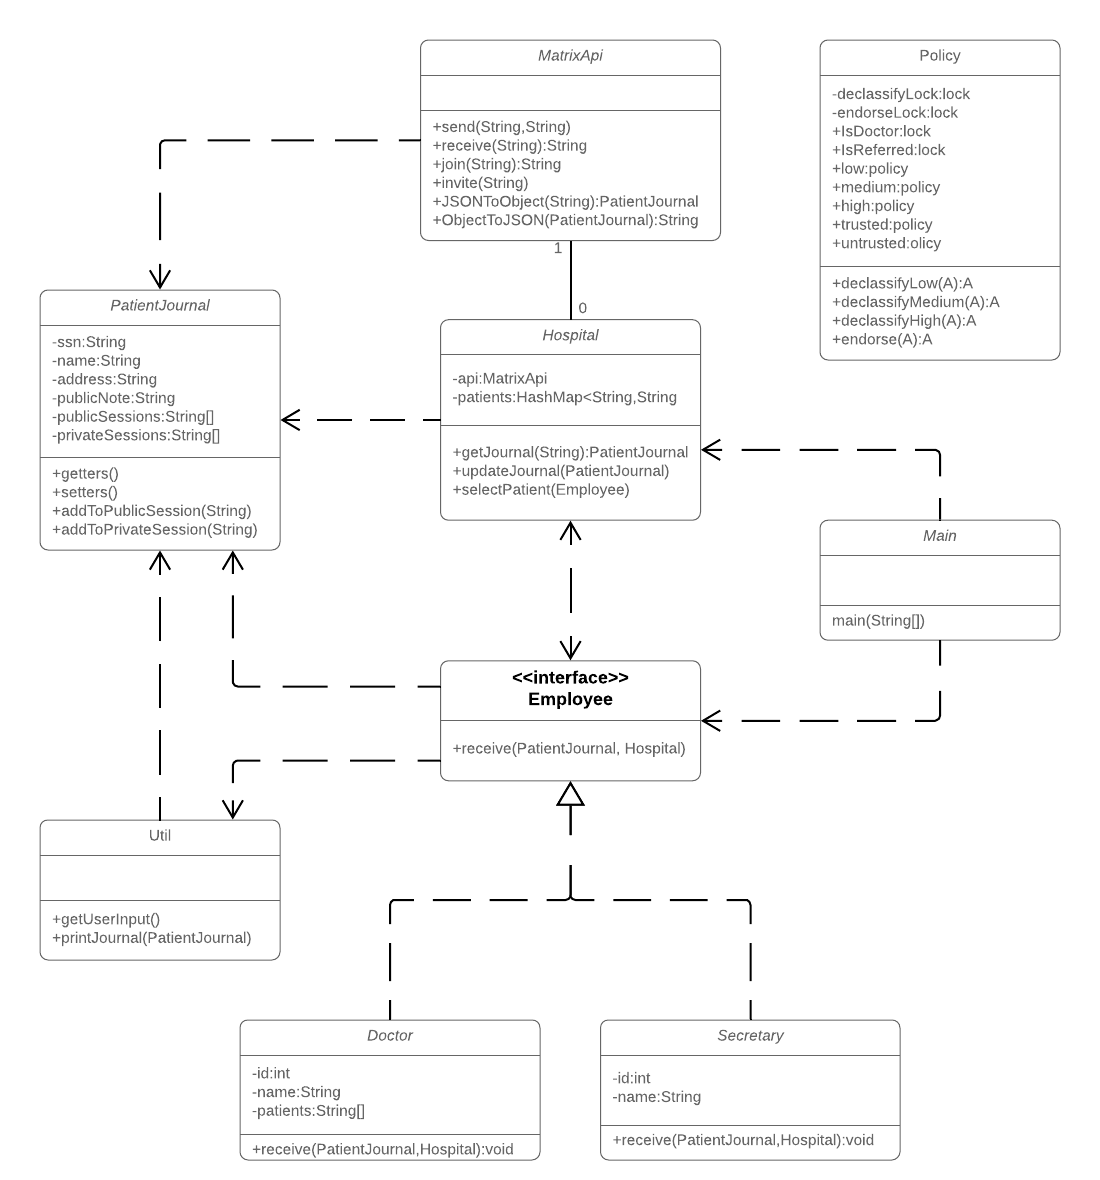
\includegraphics[width=14cm]{figures/journalsystem_class.png}
	\caption{Class diagram for the Journal system}
	\label{fig:journalsystem}
\end{figure}





\subsubsection{Limitations} \label{concurrentwrites}

%Incompatibility with Paragon


A design problem is the concurrent writes to a journal from multiple hospital. Before writing to a journal; the latest version of the journal in Matrix is first retrieved and then the writes are appended to the journal. However multiple hospitals might have retrieved the latest journal and different doctors might have committed changes to the journal and send it to Matrix hence one of the writes would be lost since only the latest journal is retrieved. A solution to this would be extending the rooms with version control functionality that would track and combine the changes made to a journal.


% It is assumed that a version control mechanism is in place and the latest journal received is always up to date.
% Solution merging data like version control systems like git.

\section{Paragon implementation}

\subsection{Matrix API}

The Matrix API implementation was briefly described in section \ref{systemdesign}. The API is implemented in Java using the foreign language binder JPY to leverage the Matrix Python SDK and makes it possible to use it with Java/Paragon. Without the API it would not be possible to use Matrix with Paragon. To be able to use the API; a Paragon \emph{signature} must be provided. In fact a signature file has to be specified to use any external Java class. The \emph{MatrixApi} signature file is specified as such:

\begin{lstlisting}
public native class MatrixApi<policy p> {
	!p void send(?p String message, ?p String room);
	?p String retrieve(?p String room);
	?p String objectToJSON(?p PatientJournalD object);
	?p PatientJournalD JSONToObject(?p String json);
}
\end{lstlisting}

The signature file describes that the \emph{MatrixApi} class takes a type argument \emph{policy} which specifies what policy the API should enforce. Note that Paragon cannot assert if the external class will respect the policies.

The annotation \emph{?} and \emph{!} represents \emph{read} and \emph{write} effects, and will be explained in the next sections.
 
\subsection{Policies}\label{policies} 

A \emph{policy-first} approach is used when implementing the prototype. The first step is to carefully specify the policies for the system. A journal has several parts that may only be obtained by appropriate users; the policies should uphold that. The policies are defined in the class \emph{Policy} and used throughout the system.

For confidentiality three policies are defined with \emph{low} being the most liberal, \emph{High} being the most strict and \emph{medium} in the middle. The figure \ref{fig:lattice_confidentiality} depicts a lattice for the three policies where information can only flow upwards. In the figure \emph{public} represents low, \emph{confidential} represents medium and \emph{secret} represents high. 

Based on the requirements the information labeled with secret should only be obtainable by the Doctor that the patient has been referred to. There could be defined a similar independent secret labels e.g. for information that only the patient's psychiatrist could view.  

% Show confidentiality lattice and combined lattice.

\begin{figure}[H] 
	\centering
	\includegraphics[width=6cm]{figures/lattice_confidentiality.png}
	\caption{Lattice in the system}
	\label{fig:lattice_confidentiality}
\end{figure}

The lattice in figure \ref{fig:lattice_confidentiality}b illustrates the integrity policy and states that data labeled as \emph{untrusted} can not flow to \emph{trusted}. The trusted and untrusted labels serves the purpose of disallowing flows to the journal.

The fields in the PatientJournal class are decorated with a combination of confidentiality labels. The \emph{product lattice} is illustrated in the figure \ref{fig:lattice_product}.

\begin{figure}[H] 
	\centering
	\includegraphics[width=7cm]{figures/lattice_product.png}
	\caption{Product lattice}
	\label{fig:lattice_product}
\end{figure}


The next section will show how the policies have been defined and used in paragon. 





\subsubsection{Defining policies}\label{policydef}
In Paragon a policy defines what actor information can flow to and under what conditions 
\cite{paragonprogramming}. Any object can be used as an actor. The confidentiality policies in the prototype uses \emph{Doctor} and \emph{Secretary} as actors. 

The policies \emph{low}, \emph{medium} and \emph{high} are defined as this:

\begin{lstlisting}
public static final policy low = { Doctor d: ;Secretary s:};
public static final policy medium = { Doctor d:};
public static final policy high = { Doctor d: IsReferred(d)};
\end{lstlisting}


Here policy \emph{low} is less restrictive than \emph{medium} since a variable labeled with the policy low can be viewed by the any\emph{Doctor} or \emph{Secretary} actor whereas a variable labeled with \emph{medium} can only be viewed by any \emph{Doctor} actor. The policy \emph{high} is a more interesting policy. It is more restrictive since it can only flow to a specific \emph{Doctor} if the lock \emph{IsReferred(d)} is open. Policy \emph{high} is an example of a dynamic policy which uses a parameterized unary lock.

The following are integrity policies defined as follows:
\begin{lstlisting}
private static final Object untrustedObserver = new Object();
private static final Object trustedObserver = new Object();
public static final policy untrusted = { untrustedObserver :; };
public static final policy trusted = { untrustedObserver :; trustedObserver: };
\end{lstlisting}


The actors used here are \emph{untrustedObserver} and \emph{trustedObserver}. The policy \emph{trusted} can be viewed by both observers while \emph{untrusted} can only be viewed by \emph{untrustedObserver}. This captures integrity since a variable labeled with \emph{untrusted} can not flow to \emph{trusted}. Note that actors used here are instances of objects and using them as actors gives the policies a special property of being combinable with other policies \cite{paragonprogramming}.


% The policies defined for confidentiality are with fresh actors and the objects correspond to the entities where information may flow. By using fresh actors the policies can be combined with other policies that would otherwise have interfered with eachother. The integrity policy is more general in nature and has defines two actors; trusted and untrusted observers. The policies are defined as follows: ?(Policy.high + Policy.trusted).

% Dynamic policy is used for when a doctor adds notes to session. The lock IsDoctor must be open for the method addToSession() can be invoked. This is checked at runtime as seen in the code snippet:


% Policy definition
% Policy usage
\subsubsection{Using policies}
A policy is used as a label on variables. To express concerns for both confidentiality and integrity the policies described previously can be combined and labeled on variables. Fields in the class \emph{PatientJournal} are defined as:

\begin{lstlisting}
	private ?(Policy.low    + Policy.trusted) String   publicNote;
	private ?(Policy.medium + Policy.trusted) String[] publicSessions;
	private ?(Policy.high   + Policy.trusted) String[] privateSessions;
\end{lstlisting}

The \emph{PatientJournal} class has methods that adds a session to \emph{publicSession} or \emph{privateSession}. The class also implements simple getter and setter methods. Common for these methods are they must specify the \emph{read} or \emph{write} effect for the method.

% Show table of policies and how they are defined and how they are used for low, high and medium.



\subparagraph{Read effects}
The read effect specifies what the information policy is. It has already been introduced when labeling the fields in the \emph{PatientJournal} class. When decorating a method with a read effect signature it simply tells what the policy is for the returned type. Paragon ensures that the policy returned must respect the policies of the field or parameters that are in the context of the method. Through read effects explicit flows are captured across methods and fields. This is an example of how a simple \emph{get()} method is defined in \emph{PatientJournal}.
\begin{lstlisting}
?(Policy.medium + Policy.trusted)
public  String[] getPublicSessions(){
	return publicSessions;
}
\end{lstlisting}

If the read effect instead was \emph{?(Policy.low+Policy.trusted)} then Paragon would have caught it since the field \emph{publicSession} has a more restrictive policy. Note that is a read effect is not specified then Paragon sets the read effect as \emph{?(Object x:)} (the least restrictive policy in Paragon).

\subparagraph{Write effects}
In Paragon the write effect prevents implicit flows. The write effect specifies what context the method can be called in. The context would have to at least as restrictive as the method write effect. The write effect for a method is defined like this:

\begin{lstlisting}
!(Policy.low + Policy.trusted) 
public void setPublicNote(?(Policy.low + Policy.trusted) String note){
	this.publicNote = note;
}
\end{lstlisting}

This method has the write effect \emph{!(Policy.lowD+Policy.trusted)}. Now if this method was called in a method that has the write effect \emph{!(Policy.highD+Policy.trusted)} then there would be an implicit flow and Paragon would detect it.

Read and write effects are important aspect of Paragon since they ensure secure information flow across methods and fields.

\subsection{Locks}
The integrity policy ensures that no information can not flow from untrusted source to variables labeled with \emph{trusted}. However we also want to specify which actors are allowed to change information. A secretary should only be able to edit the field \emph{publicNote} in \emph{PatientJournal}. A doctor should be able to add sessions to \emph{publicSessions} but should only be able to add sessions to \emph{privateSessions} if the patient is referred to the Doctor. This has been achieved through locks. The lock \emph{IsReferred} was introduced when defining the \emph{high} policy. The lock takes a \emph{Doctor} as parameter and becomes open for the doctor. Another parameterized lock is the\emph{IsDoctor} lock that opens during program start if the user is a doctor. The locks are accompanied with 0-ary locks \emph{ReferredLock} and \emph{DoctorLock}. The locks are defined as the following: 

\begin{lstlisting}
public static ?(lowD+trusted) lock IsReferred(Doctor); 
public static ?(lowD+trusted) lock ReferredLock;
public static ?(lowD+trusted) lock IsDoctor(Employee);
public static ?(lowD+trusted) lock DoctorLock;
\end{lstlisting}

The locks \emph{ReferredLock} and \emph{DoctorLock} are used on methods with a special annotation that specifies that the method can only be called if the lock is open. By using lock combined with the annotation the requirement for modifying information can be fulfilled. The class \emph{PatientJournal} provides two methods for adding sessions with the annotation:

\begin{lstlisting}
~Policy.DoctorLock
public !(Policy.mediumD + Policy.trusted) void addToPublicSessions(?(Policy.mediumD + Policy.trusted) String session){
// Add sessions
} 

~Policy.Referred
public !(Policy.highD + Policy.trusted) void addToPrivateSessions(?(Policy.highD + Policy.trusted) String session){
// Add sessions
} 	
\end{lstlisting}  

The lock \emph{DoctorLock} is opened when \emph{IsDoctor} is opened and the lock \emph{ReferredLock} opens when \emph{IsReferred} is open. 

% How a lock is opened 
The Paragon compiler might not be able to infer if the lock is opened through compilation. Hence the lock must be checked at run-time and used like this:

\begin{lstlisting}
if(Policy.IsReferred(self)){
	journal.addToPrivateSession(session);
}
\end{lstlisting}



\subsection{Declassification}
A journal system must be able to view the patient journals through some output channel. Furthermore the system must take user input through an input channel to edit a journal. Hence it is necessary to \emph{declassify} information when using an output channel and \emph{endorse} information when using an input channel. The system provides mechanism for achieving this. We need to revisit the policy definitions to make this possible. 

The policy for \emph{System.out} is the least restrictive defined as \emph{?{Object a:}}.
Hence any flow using the defined policies would be rejected. Declassification of information must be done for allowing flow to \emph{System.out}. To achieve this we have to extend the policies with a lock \emph{declassifyLock}:

\begin{lstlisting}
private lock declassifyLock;
public static final policy low = { Doctor d: ;Secretary s:; Object x: declassifyLock};
public static final policy medium = { Doctor d:; Object x: declassifyLock};
public static final policy high = { Doctor d: IsReferred(d); Object x: declassifyLock};
\end{lstlisting}

After the modification the policy now states that a variable labeled with the policy can flow to any actor if the \emph{declassifyLock} is open. Thus we can specify a method that takes some value as input, opens the lock and returns the value with the least restrictive policy:

\begin{lstlisting}
?bottom
public static <A> 
A declassifyLow(?(bottom*low) A x){
	open declassifyLock {
		return x;
	}
}
\end{lstlisting}

The method expects a parameter with a policy that is at least as restrictive as the policy \emph{low} and \emph{bottom} (variable name for {Object x:}). The method opens the lock and returns the variable and has the read effect \emph{?bottom}.  We provide similar declassify methods for \emph{low} and \emph{high}. However it is an issue that a secretary could call declassify methods for \emph{medium} and \emph{high}. We can use the annotation seen in the previous section to overcome this so only the appropriate actors can declassify:

\begin{lstlisting}
~Referred
?high
public static <A> 
A declassifyHigh(?(high*low) A x){
	open declassifyLock {
		return x;
	}
}
\end{lstlisting}

The approach for endorsement is similar with an \emph{endorseLock} added to the \emph{untrusted policy} and then specifying a method that can endorse a variable.

Declassification and endorsement are methods that should be applied with great care. It should be considered who can declassify, what is declassified, where the declassification occurs and when it can occur. The table below gives an overview of this.

\begin{table}[H]
	\hspace*{-2.3cm}
	\centering
	\begin{tabular}{|l|l|l|l|l|} 
		\hline
		& Who               & What                    & Where                                                                         & When                       \\ 
		\hline
		& Anyone~           & Journal.name            & Util.printJournal()                                                           & Printing the journal       \\
		& Anyone~ ~         & Journal.ssn             & Util.printJournal()                                                           & Printing the journal       \\
		Declassification & Anyone~ ~         & Journal.address         & Util.printJournal()                                                           & Printing the journal       \\
		& Anyone~ ~         & Journal.publicNote      & Util.printJournal()                                                           & Printing the journal       \\
		& Doctor            & Journal.publicSessions  & Util.printJournal()                                                           & Printing the journal       \\
		& Doctor (Referred) & Journal.privateSessions & Util.printJournal()                                                           & Printing the journal       \\ 
		\hline
		Endorsement      & Anyone            & User input              & \begin{tabular}[c]{@{}l@{}}secretary.receive()\\doctor.receive()\end{tabular} & After prompting for input  \\
		\hline
	\end{tabular}
\end{table}



%\subsubsection{Lattice}

\subsection{Limitations}

\subsubsection{Matrix API}

When a journal is passed to the API the encryption is not performed until the Python code is executed. Hence there exists a layer between Paragon and Matrix where the data is unencrypted and where Paragon policies cannot be enforced. This could be solved by applying encryption before passing data on to the API and have assurance of confidentiality throughout the system.

\subsubsection{Exception handling}
Another limitation of the prototype is that exceptions are unexplored. Any exception is a potential channel for implicit flows. The tools provided by Paragon such as read effects, write effects and locks can be used to properly handle exception.


\subsection{Concurrency}
Concurrency is not supported in Paragon and has been identified as an area for future work \cite{paragonpaper}. The lock used for declassification and endorsement would be affected in a concurrent system. The declassification method uses a lock that can only be opened in the same method without side effects. However in a concurrent system there could be side effects.


\section{Summary}
This chapter has described requirements for the prototype, the overall system design and how it is implemented in Paragon. We have seen how the policies can be described and enforced in Paragon. 

\chapter{Discussion}\label{discussion}
The previous section applied Paragon as a programming language and demonstrated how policies can be defined and enforced. Hence achieving stronger security guarantees. This chapter evaluate the programming experience in Paragon with Matrix and considers what Information-Flow Control offers to the prototype.

\section{Paragon}

Programming in a Information-Flow Control can be a challenging task. Paragon provides secure information flow by defining policies and labeling variables and methods. It forces the programmer to change its mindset and have more concern about the flow of information in the system. 

\subsection{Defining policies} The policy language in Paragon is flexible and expressive. The same policy can be expressed in several ways. Consider the policies for high and low: 

\begin{lstlisting}
Object observer = new Object();
Object highObserver = new Object();

policy lowA = {Object x:};
policy highA = {:};

policy lowB = {Object x:};
policy highB = {observer:};

policy lowC = {Secretary s:; Doctor d:};
policy highC = {Doctor d:};
\end{lstlisting}

Each encoding of the low and high policies has some differences e.g. \emph{lowA} has the least restrictive policy while \emph{lowC} allows flows to any doctor or secretary. Even though \emph{lowC} is low it is encoded in such way that it cannot flow to an output channel without declassification. 
There are even more possibilities when introducing locks as seen in the prototype. The prototype relies heavily on locks as for enabling declassification and endorsement of information. Another important usage of locks are to ensure that method can only be called depending on the state of the lock. This is how it is guaranteed that a secretary cannot add to \emph{privateSessions} or \emph{publicSession}. This guarantee could also have been achieved by extending the integrity policies and use write effects to control what context methods can be called. 

Since policies can be defined in many ways; the task of defining policies should be done with care and consideration for what information flows should be captured by the policies.


%\subparagraph{Auto-generating interface files}
%Using external Java classes should be done with consideration since there is no guarantee that the information flow to that class will enforce the policies. However it might be necessary to use som external library. Paragon interface file must be provided to use external classes. If the interface file is not specified correctly a compile error occur. This is a fairly trivial task but in long term it might be impractical for the programmer. Auto-generation of interface files would be an attractive feature.


\subsection{Matrix}

In the evaluation of Matrix security we found that Matrix is capable of having several security properties such as confidentiality, integrity, forward and backward secrecy which is achieved through the end-to-end encryption.

Matrix primary use case is as a secure messaging protocol however it has a wide range of use cases. If Matrix is used as a secure communication channel like in the use case for IoT described in section \ref{endtoend}, then the end-to-end encryption is not enough to achieve confidentiality and integrity throughout the system. Information-Flow Control is a mechanism that aid in achieves stronger security guarantee.

The interface between Matrix and Paragon makes it possible to combine the end-to-end encryption security guarantees with policy enforcement through Paragon hence achieving end-to-end security. The implementation provides the most basic methods and are fairly

It is challenging to setup and use the foreign binding tool JPY. However once becoming comfortable with JPY the interface can easily be extended with more methods from the Matrix Python SDK.

\section{The Policy system}


The prototype displays major improvements in terms of confidentiality and integrity in the system. The prototype is secure by construction and gives a guarantee that the defined policies about the information is enforced. Consider the Java code where a secretary handles a patient journal: 

\begin{lstlisting}

public class PatientJournal{

private String publicNote;
private String[] publicSessions; // Unaccessible to secretary
private String[] privateSessions; // Unaccessible to secretary

}

public class Secretary {

public void receive(PatientJoural journal){
// Perform task on journal
}

\end{lstlisting}

The Java compiler would be helpless in detecting if the secret parts of the journal are unintentionally accessed or modified. In the prototype such unintentional access or modification of information would be detected immediately by the Paragon compiler. This is a strong guarantee that Information-Flow Control tools offer.

The prototype also demonstrate improvement to an actual problem in the current journal systems. The section xx describes how the only mechanism is auditing and logging trail and clearly a mechanism for enforcing policies would be of great benefit. 

The prototype is by no means a full-fledged journal system and has some obvious limits. The prototype lacks support for concurrency and assumes that only a single user can use it at a time. The prototype does not handle the issue with concurrent writes described \ref{concurrentwrites} which is also impractical. The purpose of the prototype was to demonstrate improvements of the security guarantees provided by matrix to ensure end-to-end security by enforcing policies which the prototype has demonstrated.




\section{Summary}

With Paragon provides a flexible and expressive way of defining policies. Paragon can be used on top of Matrix through the provided interface. End-to-end security is achieved by extending the security guarantees from Matrix' end-to-end encryption with Paragon's enforcement of specified policies. This is demonstrated by implementing a prototype inspired by the Danish journal system.




\chapter{Conclusion} \label{conclusion}
The following goals were defined for the thesis:

\begin{itemize}
	\item a
	\item b
	\item c
	\item d
\end{itemize}

In section ?? we saw that a bla bla bla

Tools were analyzed and Paragon was selected.

Paragon has been applied to improve the security..

It has been demonstrated that the security is improved since ... 

The thesis contributes with an interface between Matrix and Paragon that can be used to develop end-to-end secure systems. There 

  that can be used with the Information-Flow Security tool Paragon. The 

\chapter*{Appendix}

The source code for the prototype can be found at \emph{https://github.com/Ansuddin/thesis-code-handin}

%\addcontentsline{toc}{chapter}{Appendices}

%\renewcommand{\thesection}{\Alph{section}}
%\setcounter{section}{0}
%\input{tex/Appendiks}

% The final section contains the sources of any and all references to other
% group documents, articles, books, etc.  that you used in creating this
% document.  You need to have created the file analysis.bib with
% entries for all of your sources.

\nocite{*}
\bibliographystyle{plainnat}
\bibliography{bibliography} % bibliography.bib is the bibliography file name

\end{document}
